\begin{enumerate}[label=\thesubsection.\arabic*, ref=\thesubsection.\theenumi]

\item
If the sum of the zeroes of the polynomial $P\brak{x} = 2x^2 - k\sqrt{2}x + 1$is $\sqrt{2}$, then the value of $k$ is:

\begin{enumerate}
\begin{multicols}{4}
   \item $\sqrt{2}$
   \item $2$
   \item $2\sqrt{2}$
   \item $\dfrac{1}{2}$
\end{multicols}
\end{enumerate}

\solution

For the given polynomial,
\begin{align}
P\brak{x} = 2x^2 - k\sqrt{2}x + 1
\end{align}
Comparing with $ax^2 + bx + c = 0$, we get
\begin{align}
a = 2,\quad b = -k\sqrt{2},\quad c = 1
\end{align}
From \eqref{eq:EE26BTECH11211-Prob_1.2.10},
\begin{align}
\text{Sum of roots} = -\frac{b}{a}
\end{align}
Given that the sum of the roots is $\sqrt{2}$ and $a=2$, $b=-k\sqrt{2}$,
\begin{align}
\sqrt{2}=\frac{k\sqrt{2}}{2}
\end{align}
Hence, $k=2$.

\item
If the probability of a player winning a game is 0.79, then the probability of his losing the same game is :
\begin{enumerate}
\begin{multicols}{4}
  \item $1.79$
  \item $0.31$
  \item $0.21\%$
  \item $0.21$
\end{multicols}
\end{enumerate}
\solution
\\Let A be an event and P\brak{A} be the probability of happening of event A.
$P\brak{A^c}$ be the probability of not happening of event A.
\begin{align}
P\brak{A} + P\brak{A^c} = 1
\end{align}
let A be the event of winning the game.
\\Given that P\brak{A}=0.79
\\Then the probability of his losing the game is
\begin{align}                
P\brak{A^c}=1-0.79
\end{align}
\begin{align}
P\brak{A^c} = 0.21
\end{align}
\item
 If the roots of equation $ax^2 + bx + c = 0$,$a \neq 0$ are real and equal ,then which of the following relation  is true ?                   
\begin{enumerate}
   \begin{multicols}{4}
   \item $a=\dfrac{b^2}{c}$
   \item $b^2=ac$
   \item $ac=\dfrac{b^2}{4}$
   \item $c=\dfrac{b^2}{a}$
   \end{multicols}
\end{enumerate}

\solution
\\Given equation is $ax^2 + bx + c = 0$
\\Given that the roots of the above equation are real and equal.
\\Hence, Discriminant D = 0
\\From \eqref{eq:EE26BTECH11211-Prob_1.4.10}
\begin{align}
b^2 - 4ac = 0\end{align}
\begin{align}
ac = \frac{b^2}{4}
\end{align}
Hence proved,

\item
In an A.P.,if the first term a = 7,nth term $a_n$ = 84 and the sum of first n terms $s_n = \dfrac{2093}{2}$ , then n is equal to :
\begin{enumerate}
   \begin{multicols}{4}
   \item $22$
   \item $24$
   \item $23$
   \item $26$
   \end{multicols}
\end{enumerate} 

\solution
\\Given that a = 7 , $a_n = 84$ and $s_n = \dfrac{2093}{2}$
\\From \eqref{eq:EE26BTECH11211-Prob_2.4.10} 
\begin{align}
S_n = \frac{n}{2}\sbrak{a_1 + l}
\end{align}

\begin{align}
n = 23
\end{align}

\item
If two positive integers p and q can  be expressed as $p = 18a^2b^4$ and $q = 20a^3b^2 $, where a and b are prime numbers , then LCM \brak{p,q} is :
\begin{enumerate}
\begin{multicols}{4}
\item $2a^2b^2$
\item $180a^2b^2$
\item $12a^2b^2$
\item $180a^3b^4$
\end{multicols}
\end{enumerate}
\solution
\\step 1:
 \\Prime factorization of $18 = 2\times3^2$
 \\Prime factorization of $20 = 2^2\times5$
 \\To find the lowest common Multiple \brak{\text{LCM}}, take the higest power of each prime factor involved:
 $LCM\brak{18,20} = 2^2\times3^2\times 5 = 4\times9\times5 = 180$
 \\Step 2:
 \\For the variable a: The terms are $a^2$ and $a^3 $. The highest power is $a^3$.
 \\For the variable b: The terms are $b^4$ and $b^2$ .
 The highest power is $b^4$.
 \\step 3:
 \\$LCM\brak{p,q} = 180a^3b^4$ 
\item
AD is a median of $\triangle ABC$ with vertices A\brak{5,-6},B\brak{6,4} and C\brak{0,0}.Length AD is equal to :
\begin{enumerate}
  \begin{multicols}{4}
  \item $\sqrt{68} units$
  \item $2\sqrt{15} units$
  \item $\sqrt{101} units$
  \item $10 units$
  \end{multicols}
\end{enumerate}  
\solution
\\Since AD is a median, D is the midpoint of side BC.
\\Coordinates of D:
\begin{align}D = \brak{\frac{6 + 0}{2},\frac{4 + 0}{2}} = \brak{3,2}
\end{align}
Find the length of AD using the distance formula:
\begin{center}
AD = $\sqrt{\brak{3 - 5}^2 + \brak{2 - \brak{-6}}^2}$
\begin{align}AD = \sqrt{\brak{-2}^2 + \brak{8}^2} = \sqrt{68}
\end{align}
\end{center}
\begin{align}
AD = \sqrt{68}
\end{align}
The following code generates the figure
\begin{lstlisting}[frame=single, basicstyle=\rmfamily, escapeinside={(*@}{@*)}]
(*@\makebox[\dimexpr\linewidth-2\fboxsep-2\fboxrule\relax][c]{codes/s6.py}@*)
\end{lstlisting}
\begin{figure}[ht]
    \centering
    \begin{tikzpicture}
        \node[inner sep=0pt] at (0,0)
        {
            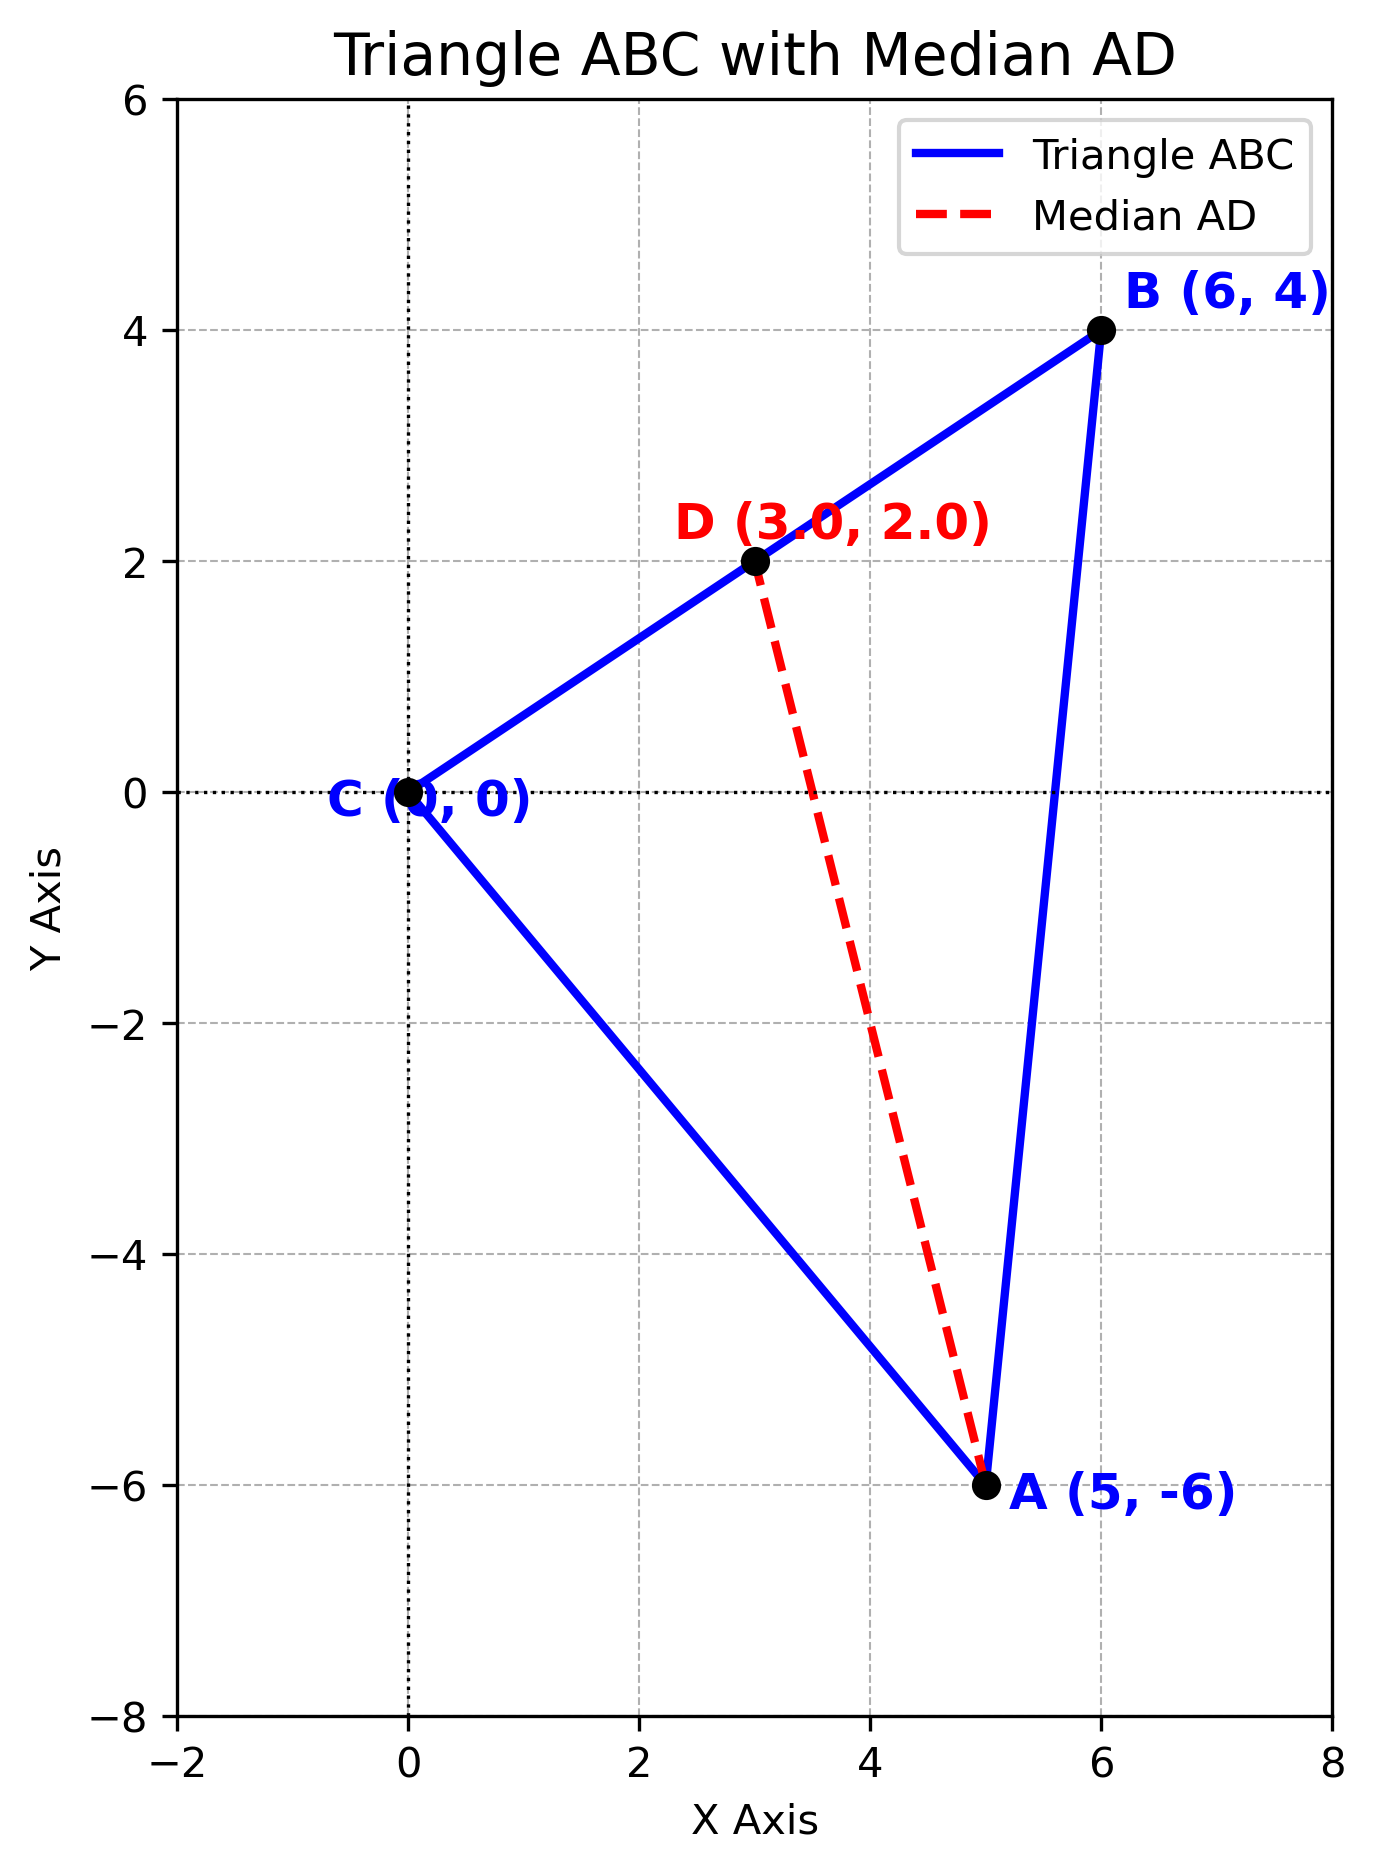
\includegraphics[
                width=0.4\textwidth,
                keepaspectratio
            ]{figs/s6.png}
        };
    \end{tikzpicture}
\end{figure}

\newpage
\item
If $sec\theta - tan\theta = m$, then the value of $sec\theta + tan\theta$ is :
\begin{enumerate}
\begin{multicols}{4}
\item $1 - \dfrac{1}{m}$
\item $m^2 - 1$
\item $\dfrac{1}{m}$
\item $-m$
\end{multicols}
\end{enumerate}

\solution
\\Given that \begin{align}
sec\theta - tan\theta = m \label{eq:EE26BTECH11211_Prob_1.4.10}
\end{align}   
 We know that 
  \begin{align}
  sec^2\theta - tan^2\theta = 1 
  \end{align}  

 \begin{align}\brak{sec\theta - tan\theta}\brak{sec\theta + tan\theta} = 1
 \end{align}
 
 From \eqref{eq:EE26BTECH11211_Prob_1.4.10}
\begin{align}m\brak{sec\theta + tan\theta} = 1
\end{align}
 \begin{align}sec\theta + tan\theta = \frac{1}{m}
 \end{align}
 
\item
From the data 1, 4, 7, 9, 16, 21, 25, if all the even numbers are removed , then the probability of getting at random a prime number from the remaining is :
\begin{enumerate}
\begin{multicols}{4}
\item $\dfrac{2}{5}$
\item $\dfrac{1}{5}$
\item $\dfrac{1}{7}$
\item $\dfrac{2}{7}$
\end{multicols}
\end{enumerate}
\solution
\\\\ Given observations are 1, 4, 7, 9, 16, 21, 25.
\\If even numbers are removed then the remaining observations are {1, 7, 9, 21, 25} N\brak{S} = 5.
\\Total no of observations that are in remaining data are 5.
\\Number of prime numbers in the remaining data is only {7} N\brak{E} = 1.
\\Probability of getting a random prime number from remaining set is
 \begin{align}
 P\brak{E} = \frac{N\brak{E}}{N\brak{S}}
\end{align}
\begin{align}P\brak{E} = \frac{1}{5}
\end{align}

\item
For some data $x_1, x_2, \ldots, x_n$ with respective frequencies
$f_1, f_2, \ldots, f_n$, the value of $\sum_{i=1}^{n} f_i \brak{x_i - \bar{x}}$ is equal to:
\begin{enumerate}
\begin{multicols}{4}
\item $n\bar{x}$
\item $1$
\item $\Sigma f_i$
\item $0$
\end{multicols}
\end{enumerate}
 \solution
 The formula for the arithmetic mean\brak{\bar{x}} of a grouped frquency distribution is given by :
 \begin{align} \bar{x} = \frac{ \sum_{i=1}^{n} f_ix_i }{ \sum_{i=1}^{n} f_i }
 \end{align}
 By cross-multiplying,we get the total sum of the data :
 \begin{align} \sum_{i=1}^{n} f_ix_i = \bar{x}\sum_{i=1}^{n} f_i 
 \end{align}
 Now, expand the given expression $\sum_{i=1}^{n} f_i \brak{x_i - \bar{x}}$ :
 \begin{align}\sum_{i=1}^{n} f_i \brak{x_i - \bar{x}} = \sum_{i=1}^{n} f_ix_i - \sum_{i=1}^{n} f_i\bar{x} 
 \end{align}
 Since $\bar{x}$ is a constant value (the mean),it can be taken outside the summation sign:
 \begin{align}\sum_{i=1}^{n} f_i \brak{x_i - \bar{x}} = \sum_{i=1}^{n} f_ix_i - \bar{x} \sum_{i=1}^{n} f_i
 \end{align}
 Substitute $ \sum_{i=1}^{n} f_ix_i = \bar{x} \sum_{i=1}^{n}f_i$ into the equation:
  \begin{align}\sum_{i=1}^{n} f_i \brak{x_i - \bar{x}} = \sum_{i=1}^{n} f_ix_i - \bar{x} \sum_{i=1}^{n} f_i = 0
  \end{align}
  Thus the sum of the deviations of a set of values from their mean is always zero.

\item
 The zeroes of a polynomial $x^2 + px + q$ are twice the zeroes of the polynomial $4x^2 - 5x - 6$. The value of p is :
 \begin{enumerate}
 \begin{multicols}{4}
 \item $-\dfrac{5}{2}$
 \item $\dfrac{5}{2}$
 \item $-5$
 \item $10$
\end{multicols}
\end{enumerate}
\solution
\\Given quadratic equations are 
\begin{align}
x^2 + px + q=0 \label{eq:EE26BTECH11211_Prob_10.1.10}
\end{align} 
\begin{align}
4x^2 - 5x - 6=0  \label{eq:EE26BTECH11211_Prob_10.2.10}
\end{align} 
\\Given that zeroes of \eqref{eq:EE26BTECH11211_Prob_10.1.10} are twice the zeroes of \eqref{eq:EE26BTECH11211_Prob_10.2.10}.
\\Sum of zeroes of equation \eqref{eq:EE26BTECH11211_Prob_10.1.10} =$ \dfrac{-p}{1}$ 
\\Sum of zeroes of equation \eqref{eq:EE26BTECH11211_Prob_10.2.10} = $-\dfrac{-5}{4}$ 
\\Since given that zeroes of \eqref{eq:EE26BTECH11211_Prob_10.1.10} are twice the zeroes of \eqref{eq:EE26BTECH11211_Prob_10.2.10}. So sum of roots of  equation \eqref{eq:EE26BTECH11211_Prob_10.1.10} are twice of sum of equations of \eqref{eq:EE26BTECH11211_Prob_10.2.10}
\\Therefore \begin{align}
\frac{-p}{1} = -2\frac{-5}{4}
\end{align}
\begin{align}
 p = -\frac{5}{2}
\end{align}

\item
If the distance between the points \brak{3,-5} and \brak{x,-5} is 15 units , then the values of x are :
\begin{enumerate}
\begin{multicols}{4}
\item $12,-18$
\item $-12,18$
\item $18,5$
\item $-9,-12$
\end{multicols}
\end{enumerate}

\solution
\\ Given two points are A\brak{3,-5} and B\brak{x,-5}.
\\ Given the distance between two points is 15 units.
\\From \eqref{eq:EE26BTECH11211-Prob_3.10}
\begin{align}
AB = \sqrt{\brak{x_2 - x_1}^2 + \brak{y_2 - y_1}^2}
\end{align}
\begin{align}
15 = \sqrt{\brak{x - 3}^2 + \brak{-5 -\brak{-5}}^2}
\end{align}

\begin{align}
x - 3 = \pm15 \label{eq:EE26BTECH11211_Prob_11.3.10}
\end{align} 
\\From \eqref{eq:EE26BTECH11211_Prob_11.3.10}
\begin{align}
 x - 3 = 15
\end{align}
\begin{align}
x = 18
\end{align}
Also from \eqref{eq:EE26BTECH11211_Prob_11.3.10}
\begin{align} 
x-3 = -15
\end{align}

\begin{align}
x = -12, 18
\end{align}

\item
If $cos\brak{\alpha + \beta} = 0$, then value of $cos\brak{\dfrac{\alpha + \beta}{2} }$ is equal to :
\begin{enumerate}
\begin{multicols}{4}
\item $\dfrac{1}{\sqrt{2}}$
\item $\dfrac{1}{2}$
\item $0$
\item $\sqrt{2}$
\end{multicols}
\end{enumerate}
\solution
\\Given that \begin{align}cos\brak{\alpha + \beta} = 0 \label{eq:EE26BTECH11211_Prob_12.1.10}
\end{align}
\\We know that \begin{align}cos\brak{\frac{\pi}{2}} = 0 \label{eq:EE26BTECH11211_Prob_12.2.10}
\end{align}  
\\Therefore from equations \eqref{eq:EE26BTECH11211_Prob_12.1.10} and \eqref{eq:EE26BTECH11211_Prob_12.2.10}
\begin{align} \alpha + \beta = \frac{\pi}{2}
\end{align}
\begin{align} \frac{\alpha + \beta}{2} = \frac{\pi}{4}
\end{align}
\\Therefore
 \begin{align}
 cos\brak{\frac{\alpha + \beta}{2}} = cos\brak{\frac{\pi}{4}} = \frac{1}{\sqrt{2}}
 \end{align}
\item
A solid sphere is cut into two hemispheres. The ratio of the surface areas of sphere to that of two hemispheres taken together, is : 
\begin{enumerate}
\begin{multicols}{4}
\item $1 : 1$
\item $1 : 4$
\item $2 : 3$
\item $3 : 2$
\end{multicols}
\end{enumerate}
\solution
\\Surface area of a sphere:
\\The total surface area of a solid sphere with radius r is:
\begin{align}\text{Surface\ Area\ of\ Sphere }= 4\pi r^2\end{align}
\\Surface Area of Two Hemispheres:
\\When a solid sphere is cut into two hemispheres, each hemisphere gets a new flat circular base.
\\The total surface area of one solid hemisphere = $3\pi r^2$.
\\Therefore, the total surface area of two hemispheres taken together is:
\begin{align}
\text{Surface\ Area\ of\ Two\ Hemispheres }= 2\times3\pi r^2 = 6\pi r^2
\end{align}
\\Finding the ratio:
\begin{align}\frac{\text{Surface\ area\ of\ sphere}}{\text{Surface\ Area\ of\ Two\ Hemispheres}} = \frac{4\pi r^2}{6\pi r^2} = \frac{2}{3}
\end{align}

\item
The volume of the largest right circular cone that can be carved out from a solid cube of edge 2 cm is :
\begin{enumerate}
\begin{multicols}{4}
\item $\dfrac{4\pi}{3}\text{\ cu\ cm}$
\item $\dfrac{5\pi}{3}\text{\ cu\ cm}$
\item $\dfrac{8\pi}{3}\text{\ cu\ cm}$
\item $\dfrac{2\pi}{3}\text{\ cu\ cm}$
\end{multicols}
\end{enumerate}
\solution
\\For the cone to be the largest possible inside a cube of edge a = 2 cm :

The diameter of the cone's base equals the edge of the cube
\\ \(\rightarrow \text{Diameter} = 2\text{ cm} \implies \text{Radius } \brak{r} = 1\text{ cm}\)
\\The height of the cone equals the edge of the cube \(\rightarrow \text{Height } \brak{h} = 2\text{ cm}\)

 The volume of a right circular cone is given by the formula:
\begin{align}V=\frac{1}{3}\pi r^{2}h
\end{align}
\\ Substitute the values into the formula:
\begin{align}V=\frac{1}{3}\times \pi \times \brak{1}^{2}\times 2=\frac{2\pi }{3}\text{\ cu\ cm}\end{align}
\begin{align}V = \frac{2\pi}{3}\text{\ cu\ cm}\end{align}
The following code generates the figure
\begin{lstlisting}[frame=single, basicstyle=\rmfamily, escapeinside={(*@}{@*)}]
(*@\makebox[\dimexpr\linewidth-2\fboxsep-2\fboxrule\relax][c]{codes/s14.py}@*)
\end{lstlisting}
\begin{figure}[ht]
    \centering
    \begin{tikzpicture}
        \node[inner sep=0pt] at (0,0)
        {
            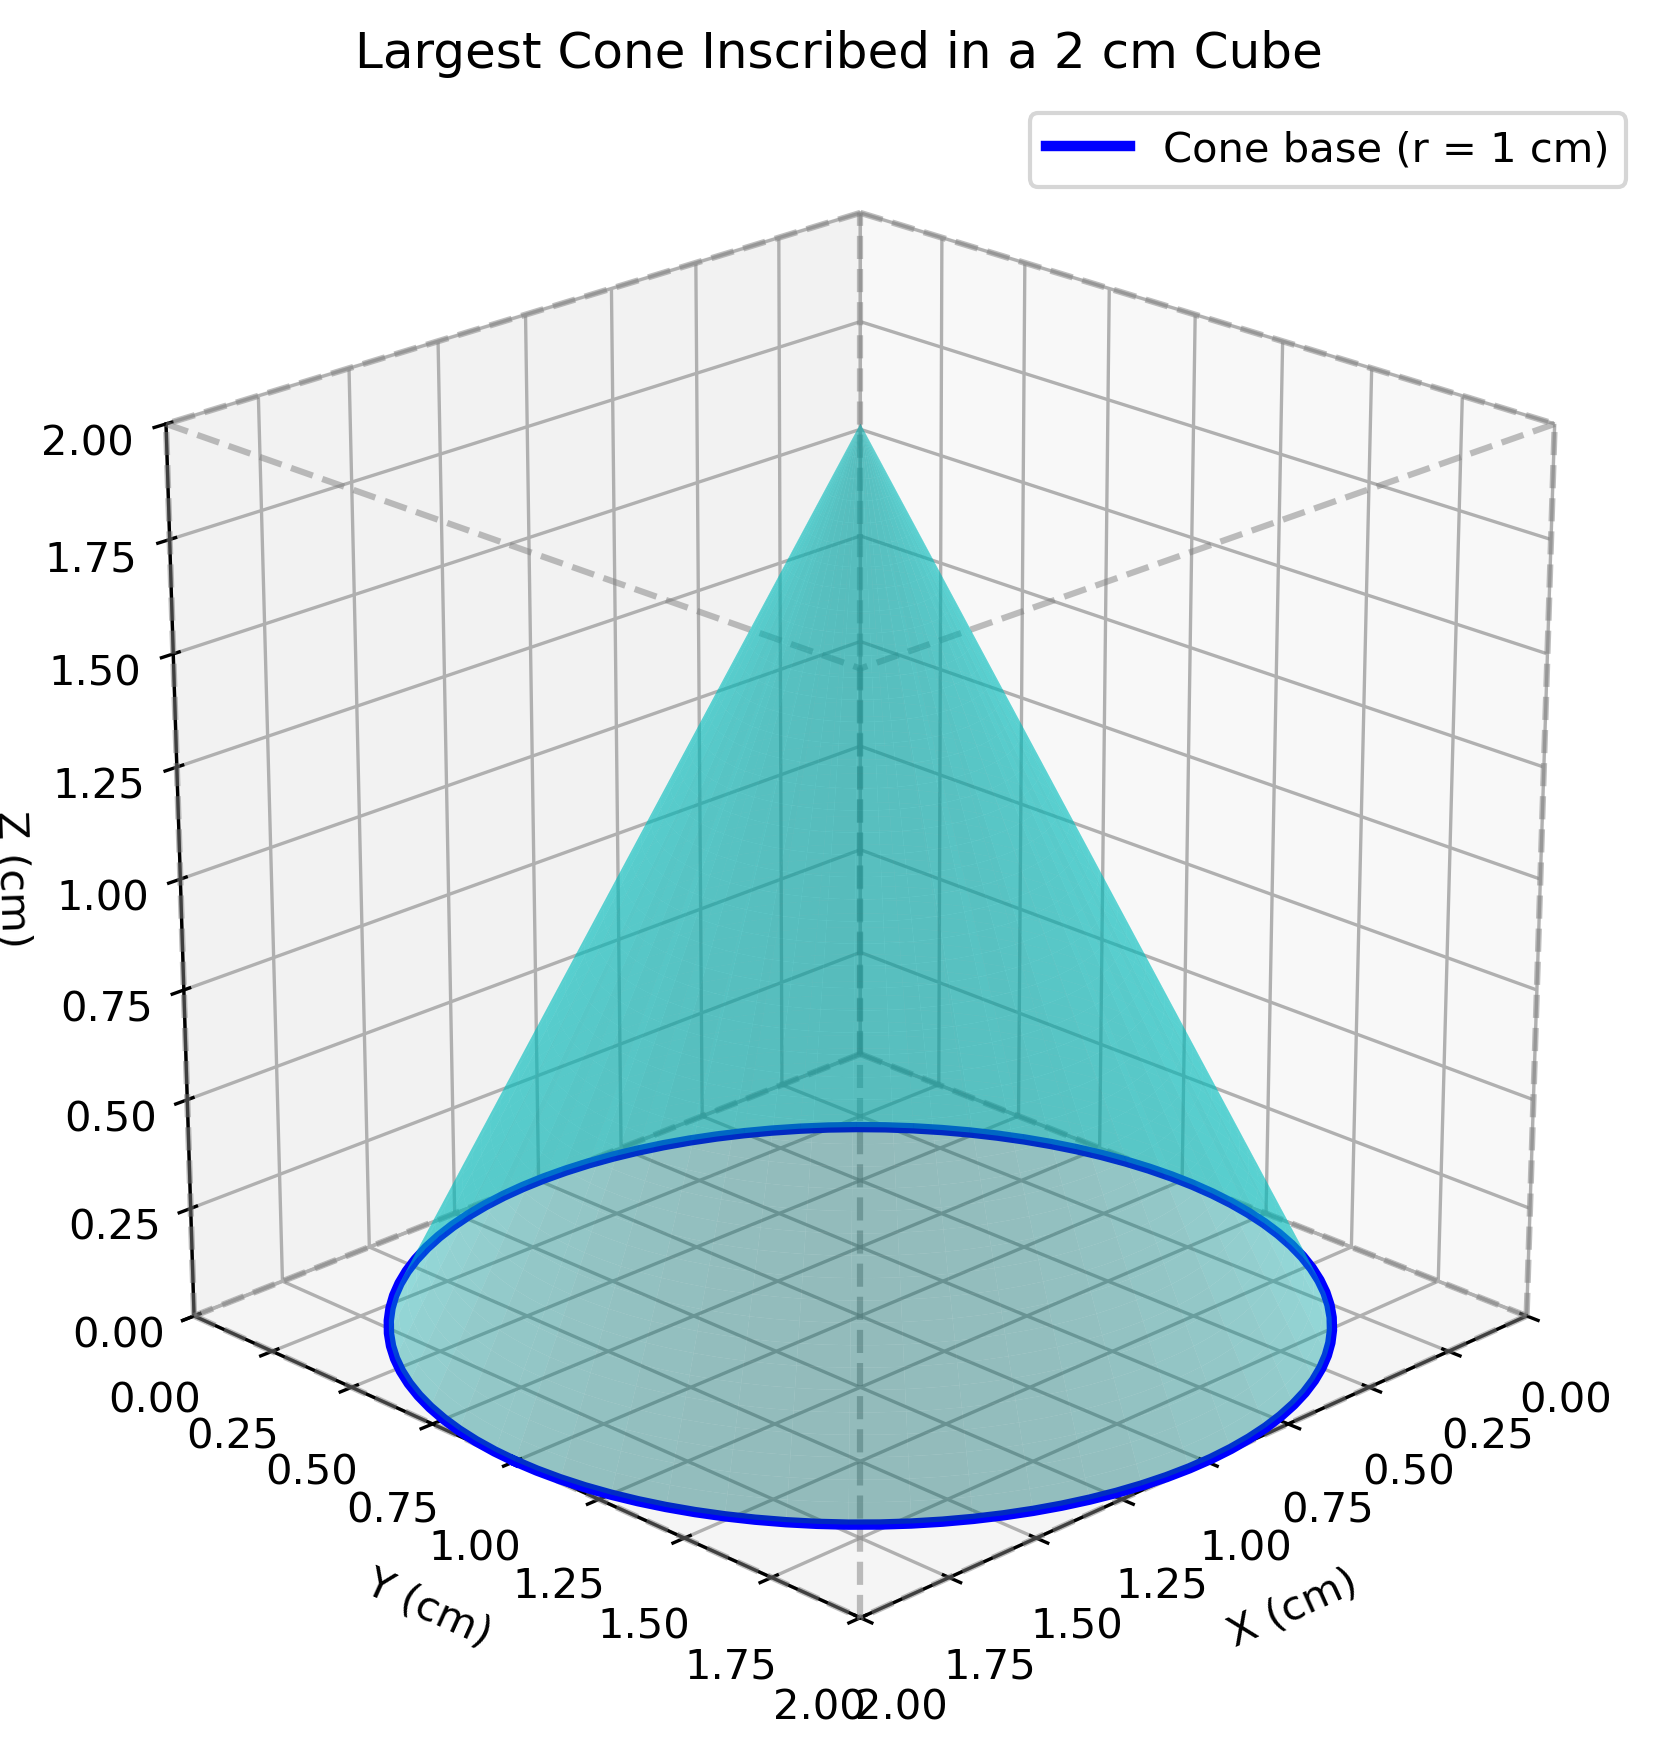
\includegraphics[
                width=0.5\textwidth,
                keepaspectratio
            ]{figs/s14.png}
        };
    \end{tikzpicture}
\end{figure}

\item
Two dice are rolled together. The probability of getting sum of numbers on the two dice as 2, 3 or 5 is:
\begin{enumerate}
\begin{multicols}{4}
\item $\dfrac{7}{36}$
\item $\dfrac{11}{36}$
\item $\dfrac{5}{36}$
\item $\dfrac{4}{9}$
\end{multicols}
\end{enumerate}
\solution

 Step 1: Find total outcomes
When two six-sided dice are rolled, the total number of possible outcomes is:

\begin{align}
\text{Total\ outcomes}=6\times 6=36
\end{align}
 Step 2: Find favorable outcomes
Let's list the pairs that give a sum of 2, 3, or 5:
\begin{align}
\text{Sum} = 2 &\implies \brak{1, 1} \quad \brak{1 \text{ outcome}} \\
\text{Sum} = 3 &\implies \brak{1, 2}, \brak{2, 1} \quad \brak{2 \text{ outcomes}} \\
\text{Sum} = 5 &\implies \brak{1, 4}, \brak{2, 3}, \brak{3, 2}, \brak{4, 1} \quad \brak{4 \text{ outcomes}}
\end{align}

\text{Total favorable outcomes} = 1 + 2 + 4 = 7
\\Probability of getting sum of numbers on the two dices as 2, 3 or 5 is 
\begin{align}P\brak{E} = \frac{\text{Total\ Favourable\ Outcomes}}{\text{Total\ Outcomes}} = \frac{7}{36}\end{align}

\item 
The centre of a circle is at \brak{2,0}. If one end of a diameter is at \brak{6,0}, then the other end is at :
\begin{enumerate}
\begin{multicols}{4}
\item $\brak{0,0}$
\item $\brak{4,0}$
\item $\brak{-2,0}$
\item $\brak{-6,0}$
\end{multicols}
\end{enumerate}
\solution
\\Given centre of the circle is \brak{2,0}.
\\Given one end of diameter is \brak{6,0}.
\\Let the other end of diameter be \brak{x,y}.
\\Therefore,
\begin{align}\brak{2,0} = \brak{\frac{x + 6}{2},\frac{y + 0}{2}}\end{align}
\begin{align}\brak{2,0} = \brak{\frac{x + 6}{2},\frac{y }{2}}\end{align}  \label{eq:EE26BTECH11211_Prob_16.2.10}
\\From \eqref{eq:EE26BTECH11211_Prob_16.2.10} equating x coordinates on both sides
\begin{align}4 = x + 6\end{align}
\begin{align}x = -2\end{align}
\\From \brak{17.1} y coordinates on both sides are equal.
\\Therefore other end of diameter of circle is \brak{-2,0}.
\\The following code generates the figure
\begin{lstlisting}[frame=single, basicstyle=\rmfamily, escapeinside={(*@}{@*)}]
(*@\makebox[\dimexpr\linewidth-2\fboxsep-2\fboxrule\relax][c]{codes/s16.py}@*)
\end{lstlisting}
\begin{figure}[ht]
    \centering
    \begin{tikzpicture}
        \node[inner sep=0pt] at (0,0)
        {
            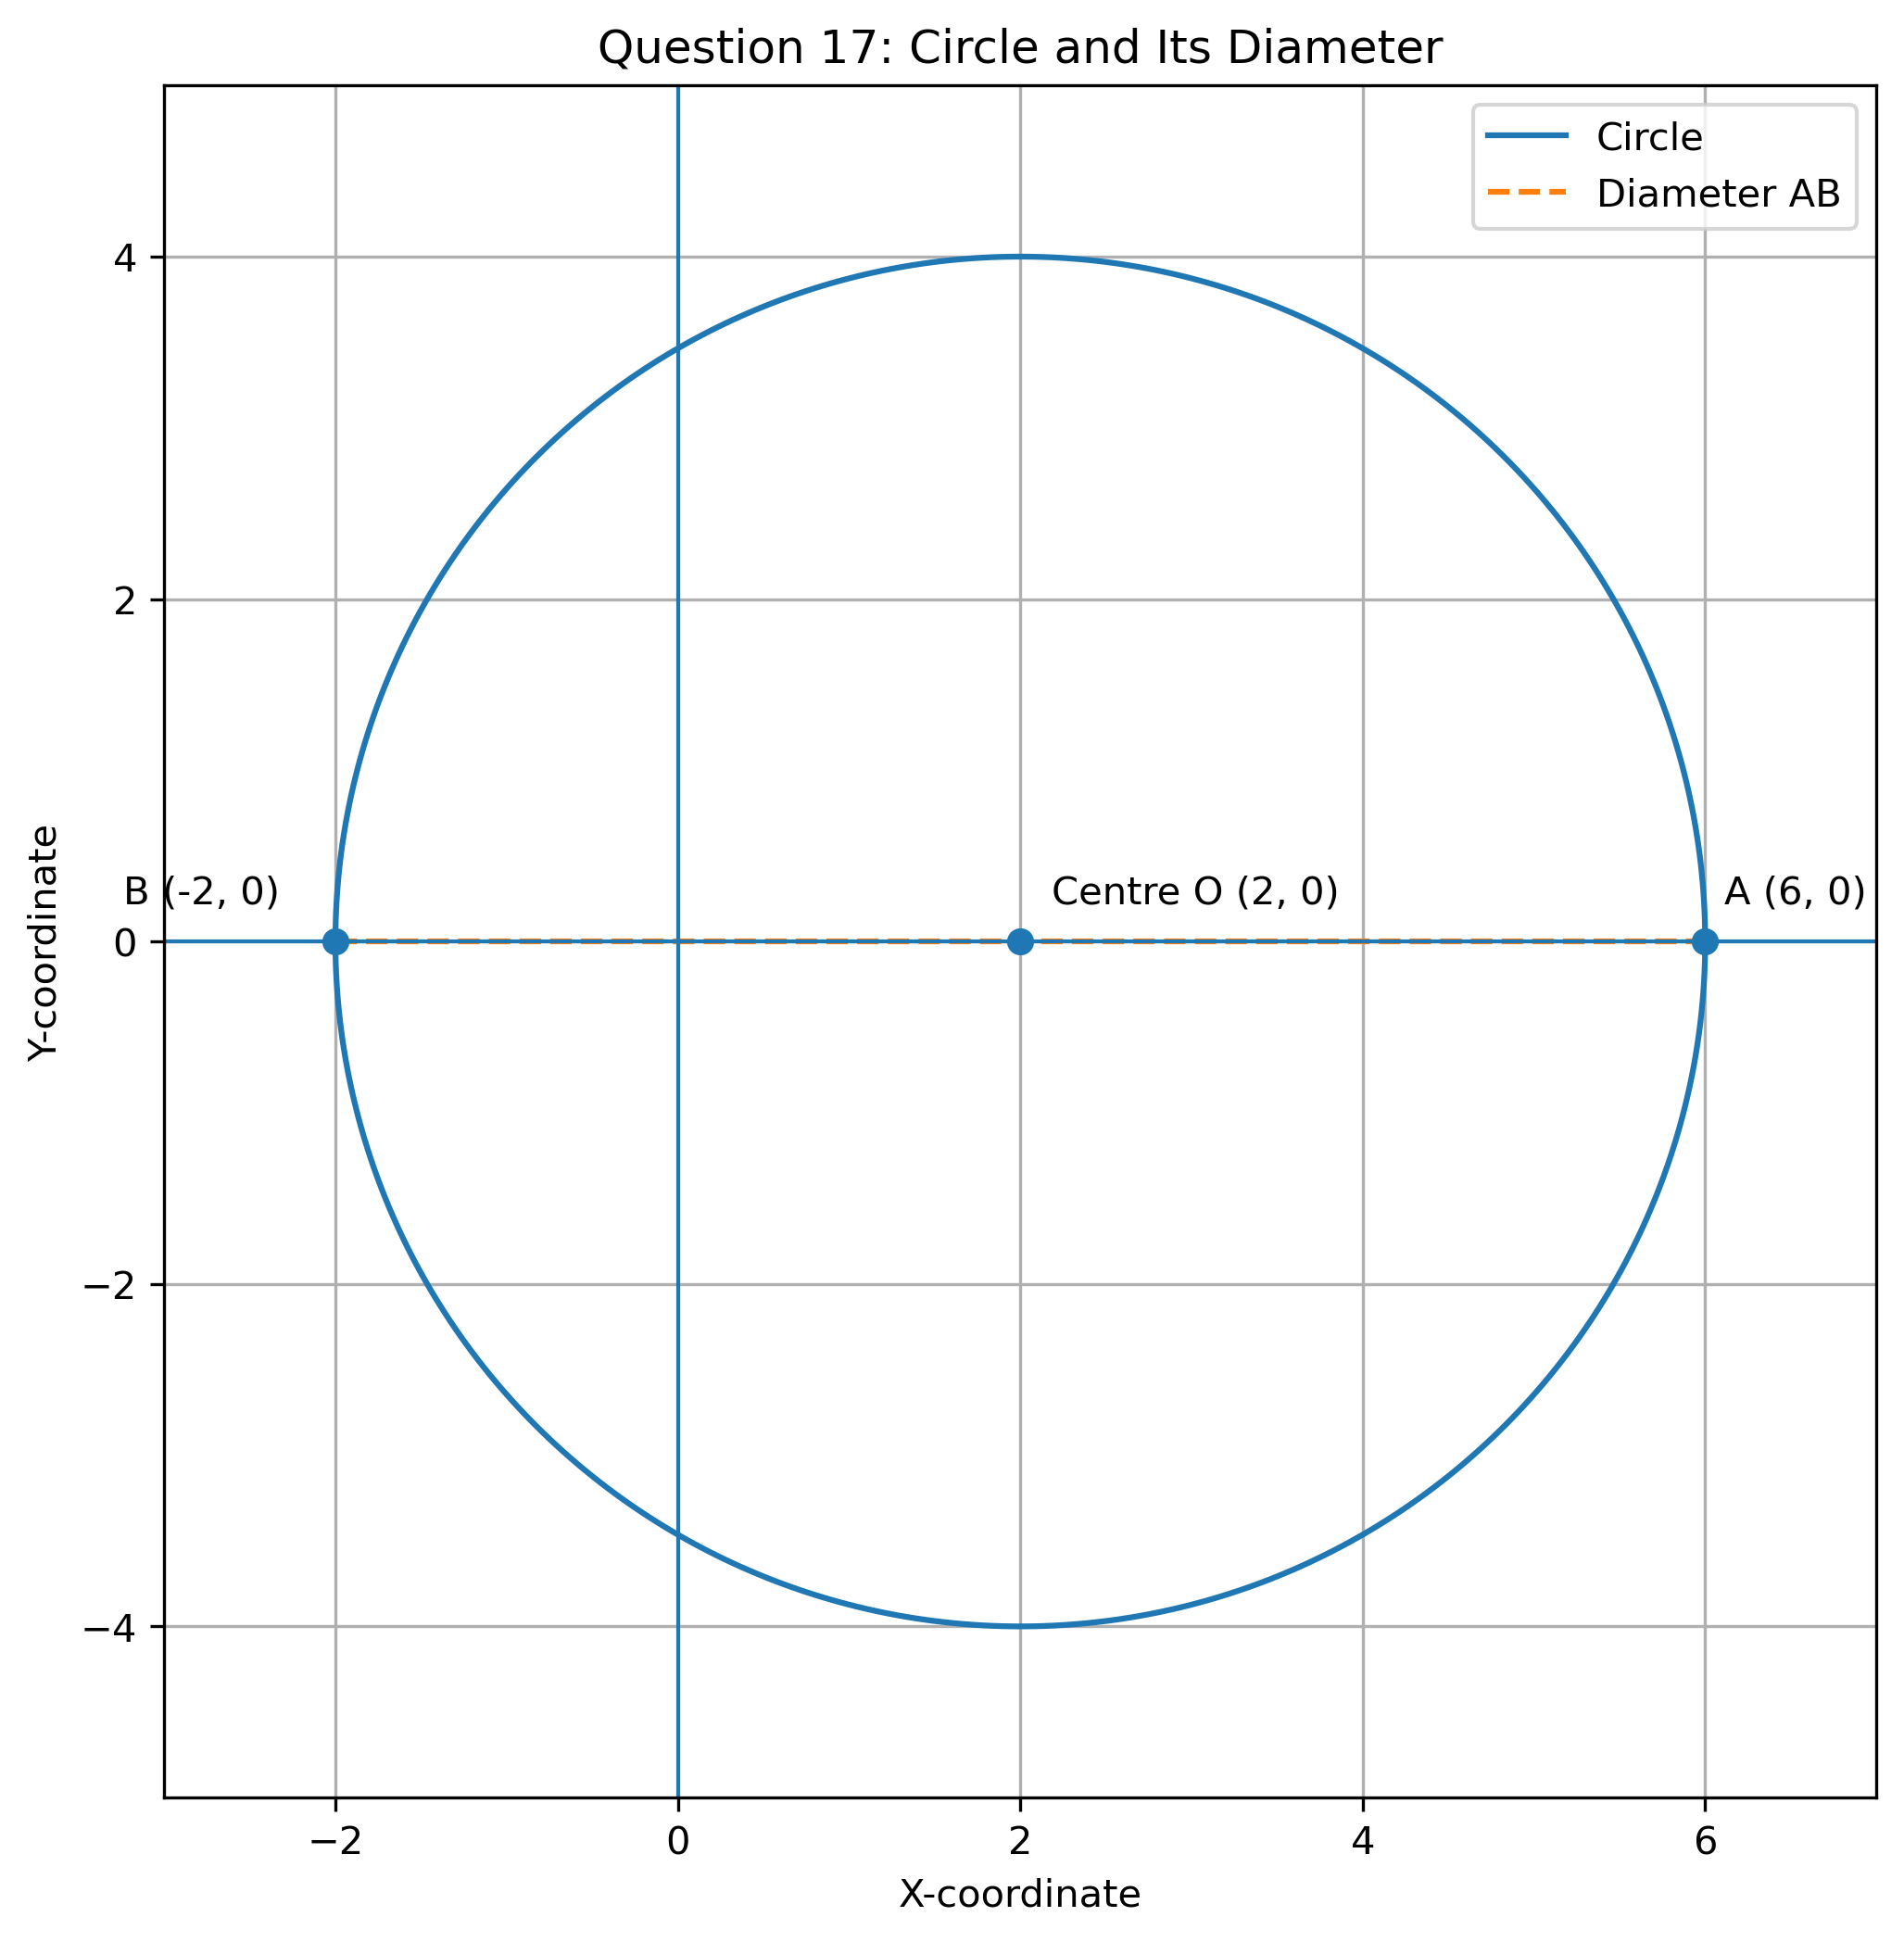
\includegraphics[
                width=0.4\textwidth,
                keepaspectratio
            ]{figs/s16.png}
        };
    \end{tikzpicture}
\end{figure}


\item
Solve the following system of linear equations 7x - 2y = 5 and 8x + 7y = 15 and verify your answer.

\solution
Given equations are
\begin{align}
7x - 2y = 5 \label{eq:EE26BTECH11211_Prob_17.1.10}
\end{align}
\begin{align}
8x + 7y = 15\label{eq:EE26BTECH11211_Prob_17.2.10}
\end{align}
Writing the equations in matrix form, we get
\begin{align}
AX=B
\end{align}
where
\begin{align}
A=\myvec{
7 & -2\\
8 & 7
},
\qquad
X=\myvec{
x\\
y
},
\qquad
B=\myvec{
5\\
15
}
\end{align}
Therefore,
\begin{align}
X=A^{-1}B
\end{align}
First, find the determinant of matrix $A$.
\begin{align}
\mydet{A}=\brak{7}\brak{7}-\brak{-2}\brak{8}
\end{align}
\begin{align}
\mydet{A}=49+16=65
\end{align}
Since $\mydet{A}\neq 0$, the inverse of $A$ exists from \eqref{eq:EE26BTECH11211_Prob_3.10.10}.

\begin{align}
A^{-1}=\frac{1}{ad-bc}
\myvec{
d & -b\\
-c & a
}
\end{align}
Hence,
\begin{align}
A^{-1}=\frac{1}{65}
\myvec{
7 & 2\\
-8 & 7
}
\end{align}
Now,
\begin{align}
X=A^{-1}B
\end{align}
\begin{align}
\myvec{
x\\
y
}
=
\frac{1}{65}
\myvec{
7 & 2\\
-8 & 7
}
\myvec{
5\\
15
}
\end{align}
Multiplying the matrices, we get
\begin{align}
\myvec{
x\\
y
}
=
\frac{1}{65}
\myvec{
7\brak{5}+2\brak{15}\\
-8\brak{5}+7\brak{15}
}
\end{align}
\begin{align}
=
\frac{1}{65}
\myvec{
65\\
65
}
\end{align}
Therefore,
\begin{align}
x=1,\qquad y=1
\end{align}
Verification:

Substituting $x=1$ and $y=1$ in \eqref{eq:EE26BTECH11211_Prob_17.1.10},
\begin{align}
7x-2y=7\brak{1}-2\brak{1}=7-2=5
\end{align}
Hence, the first equation is verified.
Substituting $x=1$ and $y=1$ in \eqref{eq:EE26BTECH11211_Prob_17.2.10},
\begin{align}
8x+7y=8\brak{1}+7\brak{1}=8+7=15
\end{align}
Hence, the second equation is also verified.
\begin{align}
 x=1,\quad y=1
\end{align}


\item
In a pack of 52 playing cards, one card is lost. From the remaining
cards, a card is drawn at random. Find the probability that the drawn
card is the queen of hearts, if the lost card is a black card.\\
\solution
\\Total number of cards in a pack = 52.
\\Since the lost card is black, the queen of hearts is still in the pack.
\\Therefore, the number of remaining cards is
\begin{align}
52-1=51
\end{align}
\\The number of queen of hearts cards remaining is 1.
\\Using the probability formula,
\begin{align}
P\brak{E}=\frac{\text{Number of favourable outcomes}}
{\text{Total number of possible outcomes}}
\end{align}
\\Hence, the required probability is
\begin{align}
P\brak{\text{Queen of Hearts}}=\frac{1}{51}
\end{align}

\item
Evaluate:
\begin{align}
2\sqrt{2}\cos 45^\circ \sin 30^\circ
+2\sqrt{3}\cos 30^\circ
\end{align}
\solution
\\We know that
\begin{align}
\cos 45^\circ=\frac{1}{\sqrt{2}},
\qquad
\sin 30^\circ=\frac{1}{2}
\end{align}
\\and
\begin{align}
\cos 30^\circ=\frac{\sqrt{3}}{2}
\end{align}
\\Substituting these values, we get
\begin{align}
=2\sqrt{2}\brak{\frac{1}{\sqrt{2}}}
\brak{\frac{1}{2}}
+2\sqrt{3}\brak{\frac{\sqrt{3}}{2}}
\end{align}
\begin{align}
2\sqrt{2}\cos 45^\circ \sin 30^\circ
+2\sqrt{3}\cos 30^\circ = 4
\end{align}

\item
If $A=60^\circ$ and $B=30^\circ$, verify that
\begin{align}
\sin\brak{A+B}=\sin A\cos B+\cos A\sin B
\end{align}
\solution
Given that
\begin{align}
A=60^\circ,\qquad B=30^\circ
\end{align}
\\Left-Hand Side (LHS):
\begin{align}
\sin\brak{A+B}=\sin\brak{60^\circ+30^\circ}=1
\end{align}
Right-Hand Side (RHS):
\begin{align}
\sin A\cos B+\cos A\sin B
\end{align}
Substituting the values of $A$ and $B$, we get
\begin{align}
=\sin 60^\circ\cos 30^\circ+\cos 60^\circ\sin 30^\circ \label{eq:EE26BTECH11211_Prob_20.1.10}
\end{align}
We know that
\begin{align}
\sin 60^\circ=\frac{\sqrt{3}}{2},
\qquad
\cos 30^\circ=\frac{\sqrt{3}}{2}
\end{align}
\begin{align}
\cos 60^\circ=\frac{1}{2},
\qquad
\sin 30^\circ=\frac{1}{2}
\end{align}
Therefore substituting the above values in \eqref{eq:EE26BTECH11211_Prob_20.1.10} we get,
\begin{align}
=\frac{\sqrt{3}}{2}\times\frac{\sqrt{3}}{2}
+\frac{1}{2}\times\frac{1}{2}&=1
\end{align}
Thus,
\begin{align}
\text{LHS}=\text{RHS}=1
\end{align}
\begin{align}
\sin\brak{A+B}=\sin A\cos B+\cos A\sin B
\end{align}
Hence, the identity is verified.


\item
In the given figure, $ABCD$ is a quadrilateral. Diagonal $BD$
bisects $\angle B$ and $\angle D$ both. Prove that:

\begin{figure}[ht]
\centering

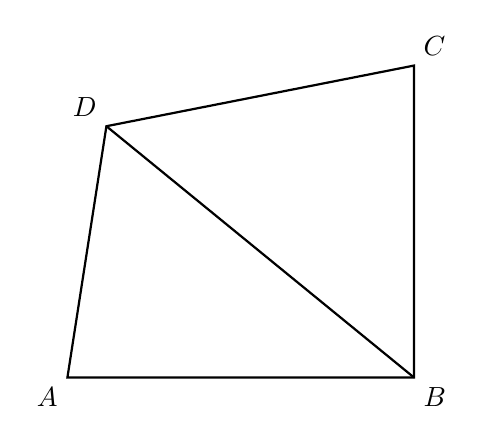
\begin{tikzpicture}[scale=1.1]

    % Vertices
    \coordinate (A) at (0,0);
    \coordinate (B) at (4,0);
    \coordinate (C) at (4,3.6);
    \coordinate (D) at (0.45,2.9);

    % Draw quadrilateral ABCD
    \draw[black, line width=0.8pt]
        (A) -- (D) -- (C) -- (B) -- cycle;

    % Draw diagonal BD
    \draw[black, line width=0.8pt]
        (D) -- (B);

    % Label vertices
    \node[below left] at (A) {$A$};
    \node[below right] at (B) {$B$};
    \node[above right] at (C) {$C$};
    \node[above left] at (D) {$D$};

\end{tikzpicture}

\end{figure}

\begin{enumerate}
    \item[\brak{a}] $\triangle ABD \sim \triangle CBD$
    \item[\brak{b}] $AB = BC$
    \end{enumerate}

\solution
\brak{a} To prove: $\triangle ABD \sim \triangle CBD$

Since $BD$ bisects $\angle B$,
\begin{align}
\angle ABD = \angle CBD 
\end{align}
Since $BD$ bisects $\angle D$,
\begin{align}
\angle ADB = \angle CDB 
\end{align}
From equations \brak{1} and \brak{2}, two angles of
$\triangle ABD$ are equal to two angles of
$\triangle CBD$ respectively.

Therefore, by the AA similarity criterion,
\begin{align}
\triangle ABD \sim \triangle CBD
\end{align}
\brak{b} To prove: $AB = BC$

Since,
\begin{align}
\triangle ABD \sim \triangle CBD
\end{align}
sides are proportional. Hence,
\begin{align}
\frac{AB}{CB} = \frac{BD}{BD}
\end{align}
Since $BD$ is the common side,
\begin{align}
\frac{AB}{CB} = 1
\end{align}
Therefore,
\begin{align}
AB = BC
\end{align}
Hence proved.

\item
 Prove that \(5-2\sqrt{3}\) is an irrational number. It is given that \(\sqrt{3}\) is an irrational number.

\solution
Let us assume that \(5-2\sqrt{3}\) is rational.

Then,
\begin{align}
5-2\sqrt{3}=r
\end{align}
where \(r\) is a rational number.

Rearranging,
\begin{align}
2\sqrt{3}=5-r
\end{align}
\begin{align}
\sqrt{3}=\frac{5-r}{2}
\end{align}

Since \(5\), \(r\), and \(2\) are rational numbers, \(\dfrac{5-r}{2}\) is also rational.

This contradicts the given fact that \(\sqrt{3}\) is irrational.
\begin{align}
 5-2\sqrt{3}\text{ is irrational.}
\end{align}
\begin{align}
\text{Hence proved.}
\end{align}

\item
Show that the number \(5\times11\times17+3\times11\) is a composite number.

\solution
Let
\begin{align}
N=5\times11\times17+3\times11
\end{align}
\begin{align}
N=968
\end{align}
Since \(968=11\times88\), the number has factors other than \(1\) and itself.
\begin{align}
 968\text{ is a composite number.}
\end{align}

\item
 Find the ratio in which the point \(\brak{\frac{8}{5},y}\) divides the line segment joining the points \(\brak{1,2}\) and \(\brak{2,3}\). Also, find the value of \(y\).

\solution
\\Let \(A\brak{1,2}\), \(B\brak{2,3}\), and \(P\brak{\frac{8}{5},y}\).
\\Let the ratio be \(m:n\).
\\Using the section formula \eqref{eq:EE26BTECH11211_Prob_3.12.10},
\begin{align}
\frac{8}{5}=\frac{2m+1n}{m+n}
\end{align}
\begin{align}
\frac{m}{n}=\frac{3}{2}
\end{align}
Therefore, the required ratio is
\begin{align}
3:2
\end{align}
Now, using the section formula for the \(y\)-coordinate,
\begin{align}
y=\frac{3\brak{3}+2\brak{2}}{3+2}
\end{align}
\begin{align}
y=\frac{13}{5}
\end{align}
\\The following code generates the figure
\begin{lstlisting}[frame=single, basicstyle=\rmfamily, escapeinside={(*@}{@*)}]
(*@\makebox[\dimexpr\linewidth-2\fboxsep-2\fboxrule\relax][c]{codes/s24.py}@*)
\end{lstlisting}
\begin{figure}[ht]
    \centering
    \begin{tikzpicture}
        \node[inner sep=0pt] at (0,0)
        {
            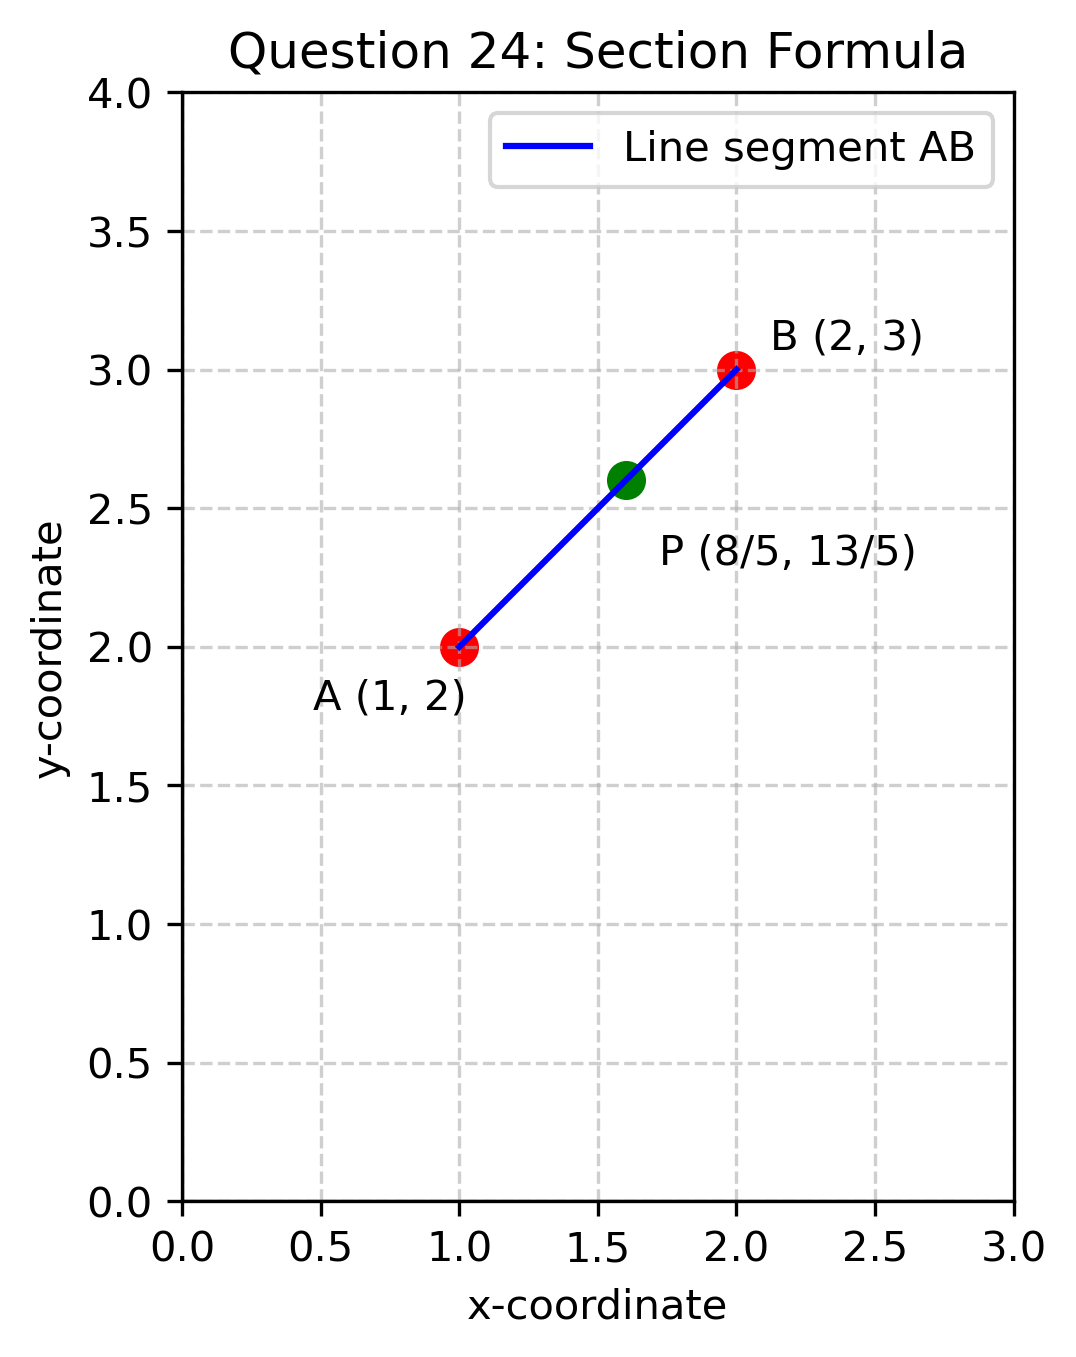
\includegraphics[
                width=0.5\textwidth,
                keepaspectratio
            ]{figs/s24.png}
        };
    \end{tikzpicture}
\end{figure}
\newpage
\item
 ABCD is a rectangle formed by the points \(A\brak{-1,-1}\), \(B\brak{-1,6}\), \(C\brak{3,6}\), and \(D\brak{3,-1}\). P, Q, R, and S are mid-points of sides AB, BC, CD, and DA respectively. Show that diagonals of the quadrilateral PQRS bisect each other.

\solution
Given:
\begin{align}
A\brak{-1,-1},\quad B\brak{-1,6},\quad C\brak{3,6},\quad D\brak{3,-1}
\end{align}
Since \(P,Q,R,S\) are the mid-points of \(AB,BC,CD,DA\), respectively, using the midpoint formula:
\begin{align}
P=\brak{\frac{-1+\brak{-1}}{2},\frac{-1+6}{2}}
\end{align}
similarly,
\begin{align}
Q=\brak{1,6},R=\brak{3,\frac{5}{2}},S=\brak{1,-1}
\end{align}
Now, the diagonals of quadrilateral \(PQRS\) are \(PR\) and \(QS\).
\\The midpoint of \(PR\) is
\begin{align}
M_1=\brak{\frac{-1+3}{2},\frac{\frac{5}{2}+\frac{5}{2}}{2}}
\end{align}
\begin{align}
M_1\brak{1,\frac{5}{2}}
\end{align}
The midpoint of \(QS\) is
\begin{align}
M_2=\brak{\frac{1+1}{2},\frac{6+\brak{-1}}{2}}
\end{align}
\begin{align}
M_2\brak{1,\frac{5}{2}}
\end{align}
Since \(M_1=M_2\), the diagonals have the same midpoint.
\begin{align}
\text{ The diagonals of }PQRS\text{ bisect each other.}
\end{align}
The following code generates the figure
\begin{lstlisting}[frame=single, basicstyle=\rmfamily, escapeinside={(*@}{@*)}]
(*@\makebox[\dimexpr\linewidth-2\fboxsep-2\fboxrule\relax][c]{codes/s25.py}@*)
\end{lstlisting}
\begin{figure}[ht]
    \centering
    \begin{tikzpicture}
        \node[inner sep=0pt] at (0,0)
        {
            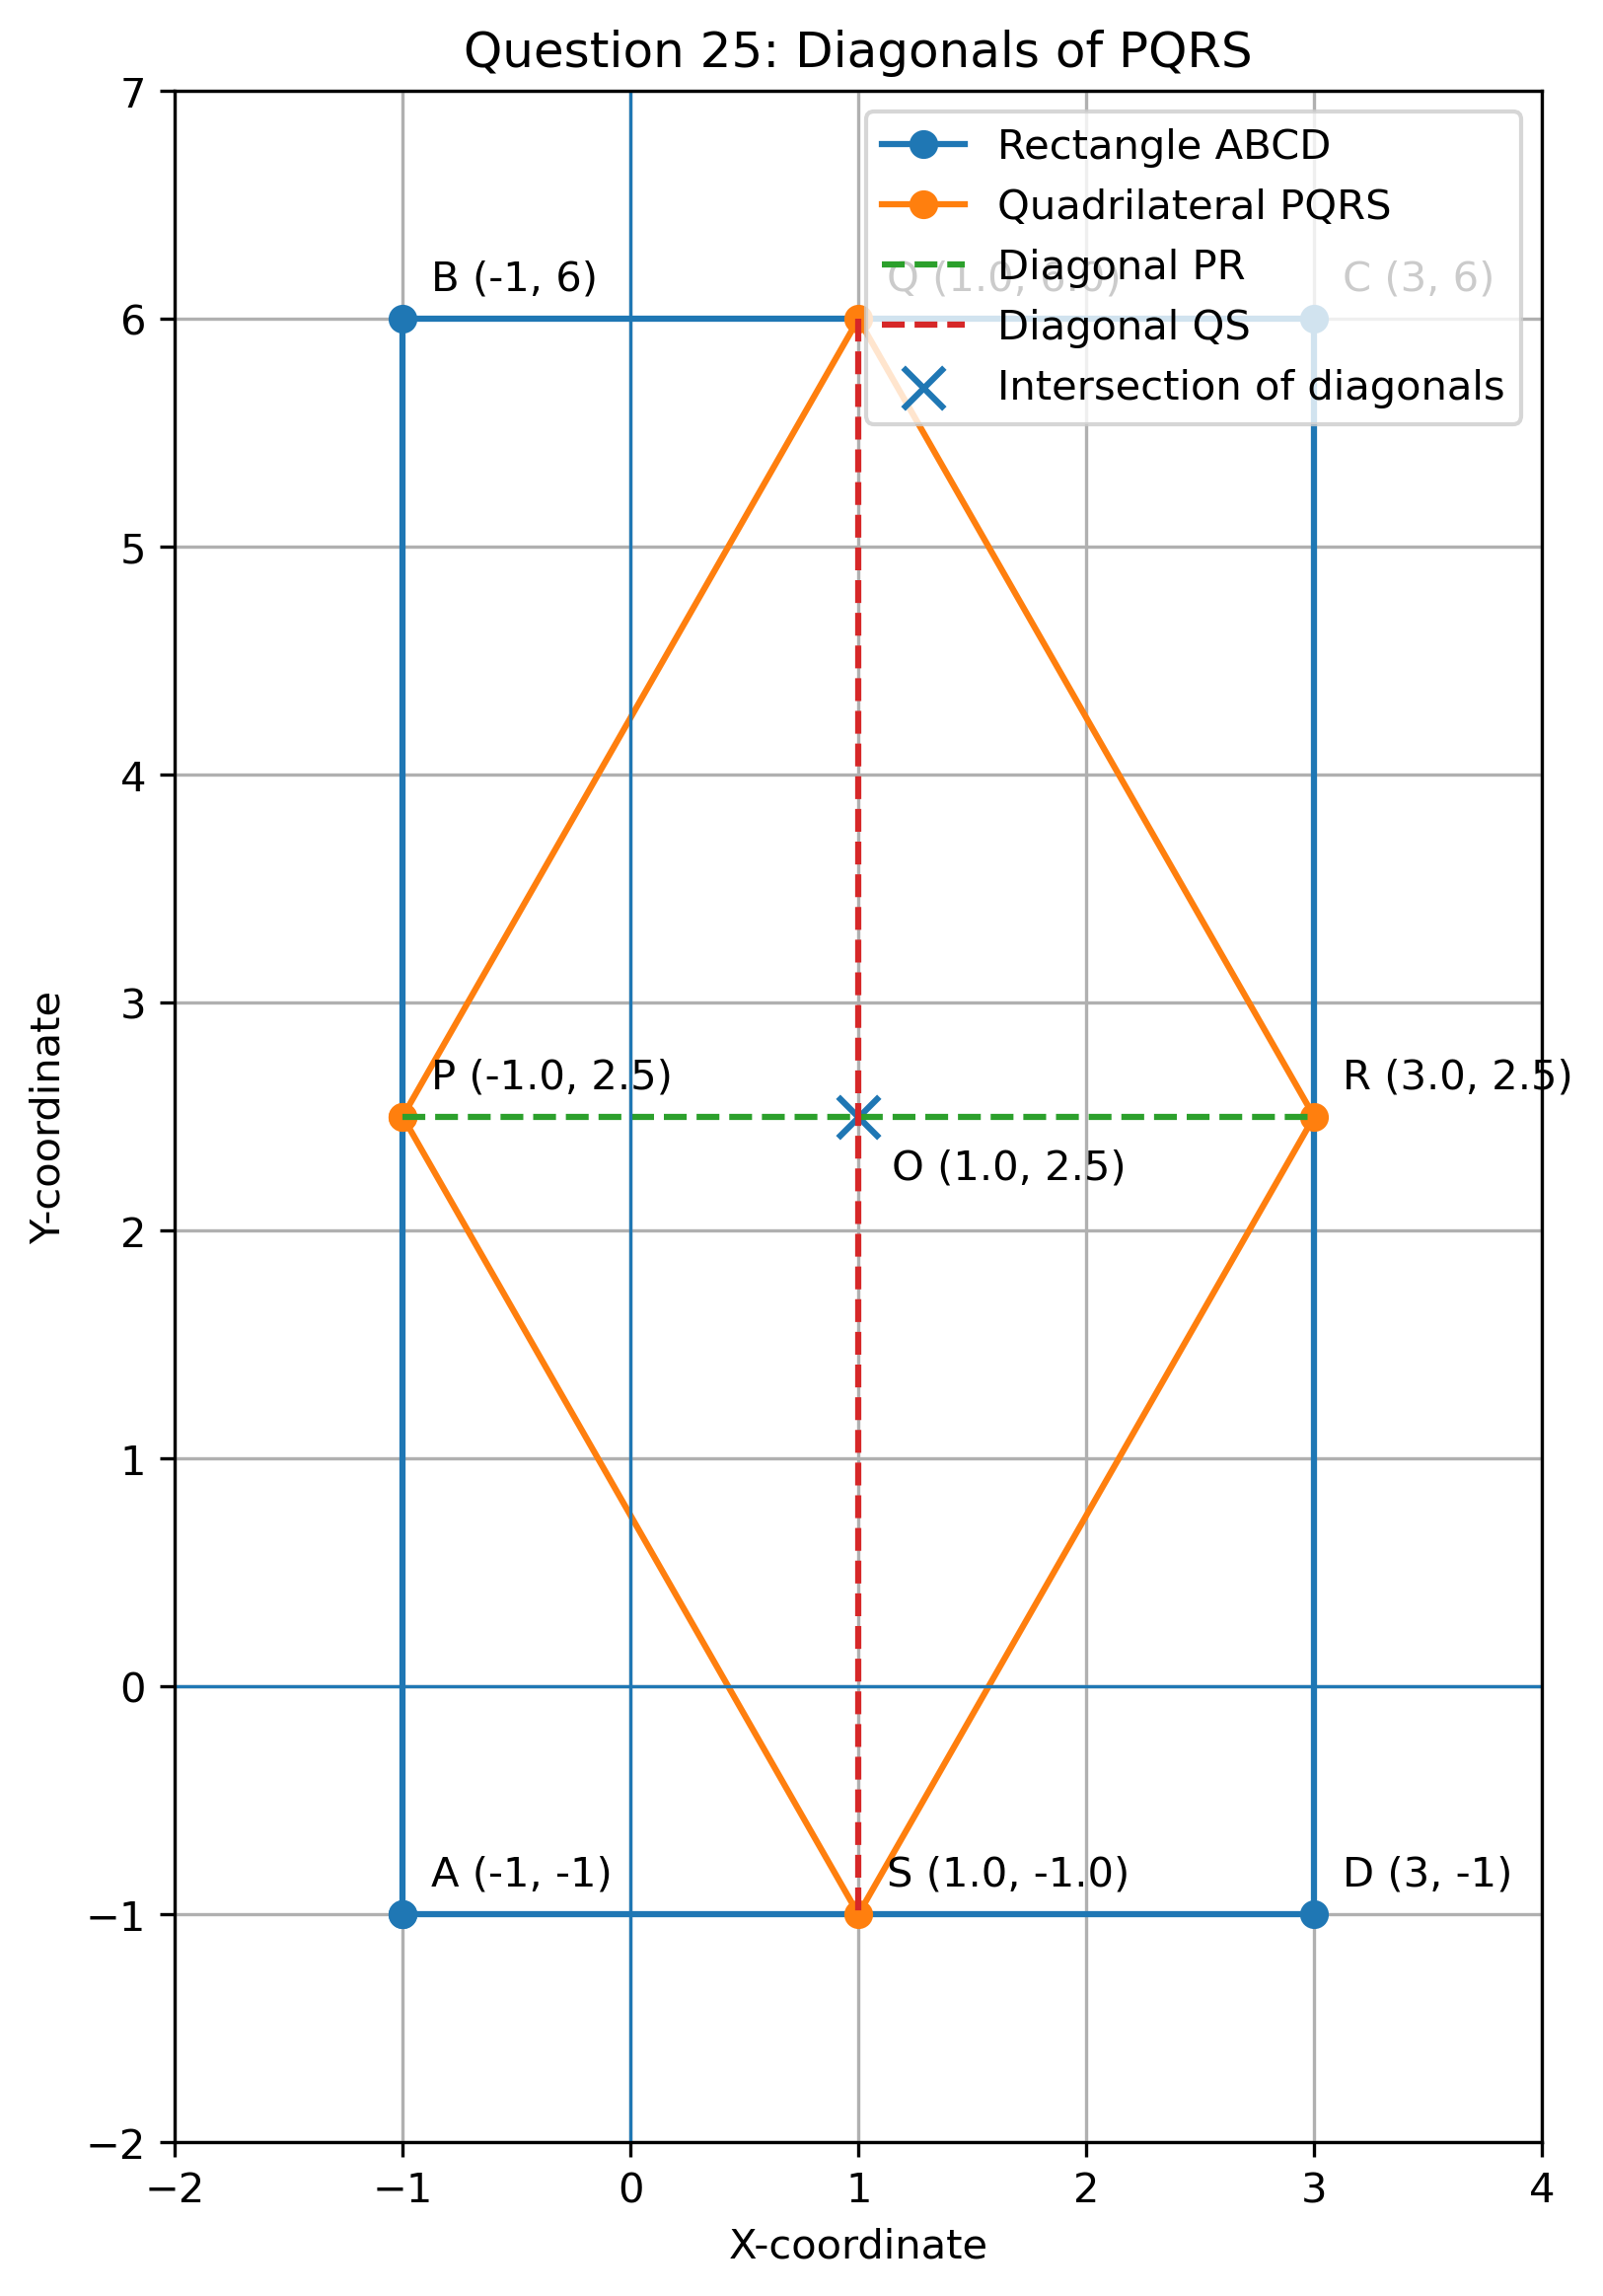
\includegraphics[
                width=0.5\textwidth,
                keepaspectratio
            ]{figs/s25.png}
        };
    \end{tikzpicture}
\end{figure}
\newpage
\item
 In a workshop, 48, 80 and 144 teachers of three different subjects are present. If each room must contain the same number of teachers and each room must contain teachers of only one subject, find the minimum number of rooms required.

\solution
To find the minimum number of rooms, we calculate the HCF of \(48\), \(80\) and \(144\).

Prime factorisation:
\begin{align}
48 = 2^4 \times 3
\end{align}
\begin{align}
144 = 2^4 \times 3^2
\end{align}
Therefore,
\begin{align}
\mathrm{HCF}\brak{48,80,144}=2^4=16
\end{align}
Hence, each room can contain \(16\) teachers.

Number of rooms required for the first subject:
\begin{align}
\frac{48}{16}=3
\end{align}
Number of rooms required for the second subject:
\begin{align}
\frac{80}{16}=5
\end{align}
Number of rooms required for the third subject:
\begin{align}
\frac{144}{16}=9
\end{align}
Total number of rooms required:
\begin{align}
3+5+9=17
\end{align}
\begin{align}
\text{Minimum number of rooms}=17
\end{align}

\item
Prove that
\begin{align}
\frac{\tan\theta}{1-\cot\theta}
+
\frac{\cot\theta}{1-\tan\theta}
=
1+sec\theta cosec\theta
\end{align}
\solution
Taking the L.H.S.,
\begin{align}
\begin{aligned}
\text{L.H.S.}
&= \frac{\tan\theta}{1-\cot\theta}
+ \frac{\cot\theta}{1-\tan\theta}
\\[8pt]
&= \frac{\tan\theta\brak{1-\tan\theta}
+\cot\theta\brak{1-\cot\theta}}
{\brak{1-\cot\theta}\brak{1-\tan\theta}}
\\[8pt]
&= \frac{\tan\theta+\cot\theta-\tan^2\theta-\cot^2\theta}
{1-\tan\theta-\cot\theta+\tan\theta\cot\theta}
\end{aligned}
\end{align}
Using \(\tan\theta\cot\theta=1\),
\begin{align}
\text{L.H.S.}
=
\frac{\tan\theta+\cot\theta-\tan^2\theta-\cot^2\theta}
{2-\tan\theta-\cot\theta}
\end{align}
Since
\begin{align}
\tan^2\theta+\cot^2\theta
=\brak{\tan\theta+\cot\theta}^2-2,
\end{align}
we obtain
\begin{align}
\text{L.H.S.}
=
\frac{\tan\theta+\cot\theta-\brak{\tan\theta+\cot\theta}^2+2}
{2-\tan\theta-\cot\theta}
\end{align}
\begin{align}
= \tan\theta+\cot\theta+1
\end{align}
Also,
\begin{align}
\tan\theta+\cot\theta
=\frac{\sin\theta}{\cos\theta}
+\frac{\cos\theta}{\sin\theta}
\end{align}
\begin{align}
=\frac{\sin^2\theta+\cos^2\theta}
{\sin\theta\cos\theta}
\end{align}
Using 
\begin{align}
\sin^2\theta + \cos^2\theta=1
\end{align},
\begin{align}
tan\theta+cot\theta = \frac{1}{\sin\theta cos\theta} = sec\theta cosec\theta
\end{align}
Therefore,
\begin{align}
\text{L.H.S.}=1+ sec\theta cosec\theta
=\text{R.H.S.}
\end{align}
Hence proved.

\item
 Three years ago, Rashmi was thrice as old as Nazma. Ten years later, Rashmi will be twice as old as Nazma. How old are Rashmi and Nazma now?

\solution
Let the present age of Rashmi be \(x\) years and the present age of Nazma be \(y\) years.

Three years ago,
\begin{align}
x-3=3\brak{y-3}
\end{align}
\begin{align}
x-3y=-6 \label{eq:EE26BTECH11211_Prob_28.1.10}
\end{align}
Ten years later,
\begin{align}
x+10=2\brak{y+10}
\end{align}
\begin{align}
x-2y=10 \label{eq:EE26BTECH11211_Prob_28.2.10}
\end{align}
Subtracting equation \eqref{eq:EE26BTECH11211_Prob_28.1.10} from equation \eqref{eq:EE26BTECH11211_Prob_28.2.10},
\begin{align}
\brak{x-2y}-\brak{x-3y}=10-\brak{-6}
\end{align}
\begin{align}
y=16
\end{align}
Substituting \(y=16\) in equation \brak{2},
\begin{align}
x-2\brak{16}=10
\end{align}
\begin{align}
x=42
\end{align}
Therefore,
\begin{align}
\text{Rashmi's present age}=42\text{ years}
\end{align}
\begin{align}
\text{Nazma's present age}=16\text{ years}
\end{align}

\item
 In the given figure, \(AB\) is a diameter of the circle with centre \(O\). \(AQ\), \(BP\) and \(PQ\) are tangents to the circle. Prove that \(\angle POQ=90^\circ\).
\begin{figure}[ht]
    \centering

    \begin{tikzpicture}
        \node[inner sep=0pt] at (0,0)
        {
            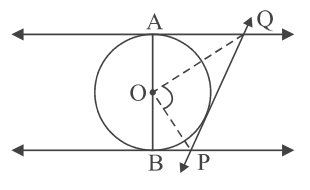
\includegraphics[
                width=0.5\textwidth,
                keepaspectratio
            ]{figs/q29.png}
        };
    \end{tikzpicture}

\end{figure}


\solution
Since \(AQ\) and \(BP\) are tangents to the circle,
\begin{align}
OA \perp AQ
\end{align}
\begin{align}
OB \perp BP
\end{align}
Therefore,
\begin{align}
\angle OAQ=90^\circ,\qquad \angle OBP=90^\circ
\end{align}
In quadrilateral \(AOBP\),
\begin{align}
\angle AOB=180^\circ
\end{align}
Since \(AB\) is a diameter, \(A\), \(O\), and \(B\) are collinear.

Using the properties of tangents drawn from an external point,
\begin{align}
QA= \text{tangent from }Q,\qquad PB=\text{tangent from }P
\end{align}
Hence, the angle between \(PQ\) and \(PO\) and the angle between \(PQ\) and \(QO\) are complementary.

Therefore,
\begin{align}
\angle POQ=90^\circ
\end{align}

\item
 A circle with centre \(O\) and radius \(8\) cm is inscribed in a quadrilateral \(ABCD\), in which \(P,Q,R,S\) are the points of contact as shown. If \(AD\perp DC\), \(BC=30\) cm and \(BS=24\) cm, find the length \(DC\).
\begin{figure}[ht]
    \centering

    \begin{tikzpicture}
        \node[inner sep=0pt] at (0,0)
        {
            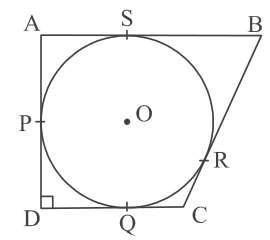
\includegraphics[
                width=0.5\textwidth,
                keepaspectratio
            ]{figs/q30.png}
        };
    \end{tikzpicture}
\end{figure}


\solution
Tangents drawn from an external point to a circle are equal.
\\From point \(B\),
\begin{align}
BS=BR=24\text{ cm}
\end{align}
Given,
\begin{align}
BC=30\text{ cm}
\end{align}
Therefore,
\begin{align}
BC=BR+RC
\end{align}
\begin{align}
RC=6\text{ cm}
\end{align}
From point \(C\),
\begin{align}
CQ=CR=6\text{ cm}
\end{align}
Since \(AD\perp DC\), and the circle has radius \(8\) cm, the tangent lengths from \(D\) to the points of contact on \(AD\) and \(DC\) are equal. Thus,
\begin{align}
DQ=DP=8\text{ cm}
\end{align}
Therefore,
\begin{align}
DC=DQ+QC
\end{align}
\begin{align}
DC=14\text{ cm}
\end{align}

\item
The difference between the outer and inner radii of a hollow right circular cylinder of length \(14\) cm is \(1\) cm. If the volume of the metal used in making the cylinder is \(176\text{ cm}^3\), find the outer and inner radii of the cylinder.

\solution
Let the outer radius be \(R\) cm and the inner radius be \(r\) cm.
Given,
\begin{align}
R-r=1
\end{align}
Therefore,
\begin{align}
R=r+1 \tag{1}
\end{align}
The volume of metal used in making the hollow cylinder is
\begin{align}
V=\pi h\brak{R^2-r^2}
\end{align}
Given \(h=14\) cm and \(V=176\text{ cm}^3\),
\begin{align}
\pi \times 14\brak{R^2-r^2}=176
\end{align}
Using \(\pi=\frac{22}{7}\),
\begin{align}
\frac{22}{7}\times14\brak{R^2-r^2}=176
\end{align}
\begin{align}
R^2-r^2=4
\end{align}
Using the identity \(a^2-b^2=\brak{a-b}\brak{a+b}\),
\begin{align}
\brak{R-r}\brak{R+r}=4
\end{align}
Since \(R-r=1\),
\begin{align}
R+r=4 \tag{2}
\end{align}
Adding equations \brak{1} and \brak{2},
\begin{align}
2R=5
\end{align}
\begin{align}
R=\frac{5}{2}=2.5\text{ cm}
\end{align}
Substituting \(R=2.5\) into \(R-r=1\),
\begin{align}
2.5-r=1
\end{align}
\begin{align}
r=1.5\text{ cm}
\end{align}
Therefore,
\begin{align}
\text{Outer radius}=2.5\text{ cm}
\end{align}
\begin{align}
\text{Inner radius}=1.5\text{ cm}
\end{align}
The following code generates the figure
\begin{lstlisting}[frame=single, basicstyle=\rmfamily, escapeinside={(*@}{@*)}]
(*@\makebox[\dimexpr\linewidth-2\fboxsep-2\fboxrule\relax][c]{codes/s31.py}@*)
\end{lstlisting}
\begin{figure}[ht]
    \centering

    \begin{tikzpicture}
        \node[inner sep=0pt] at (0,0)
        {
            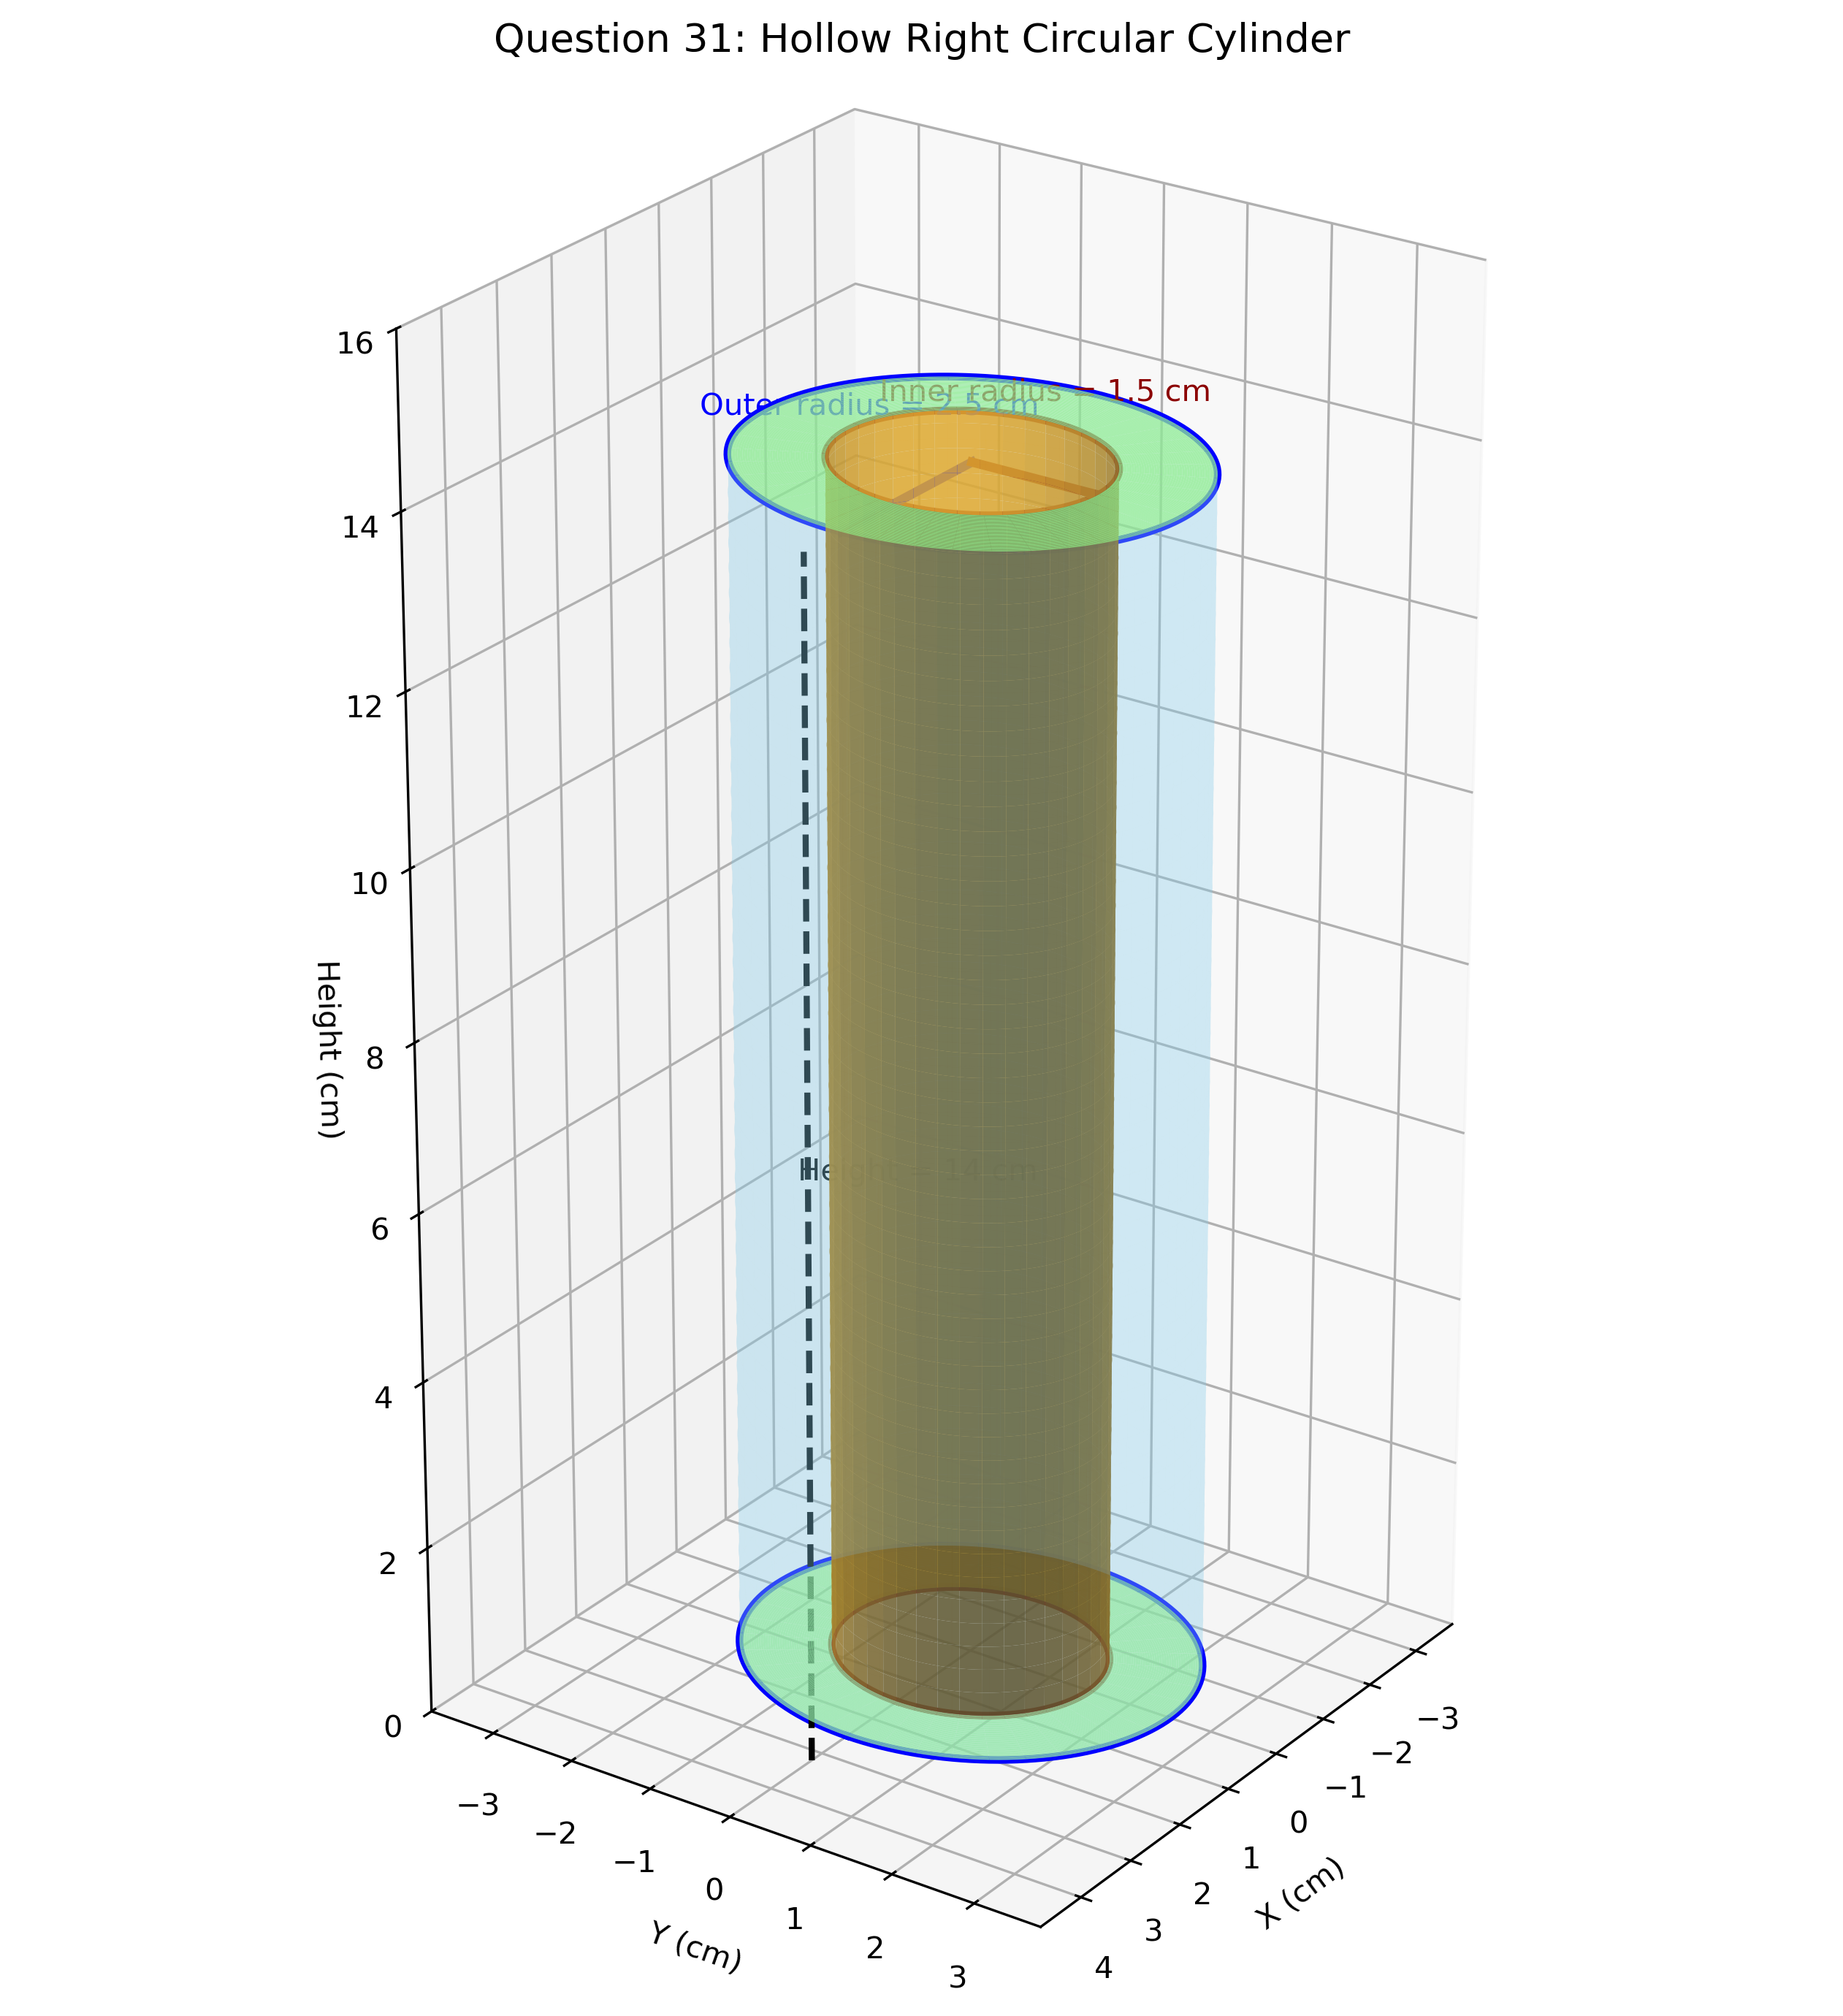
\includegraphics[
                width=0.5\textwidth,
                keepaspectratio
            ]{figs/s31.png}
        };
    \end{tikzpicture}
\end{figure}


\item
 An arc of a circle of radius \(21\) cm subtends an angle of \(60^\circ\) at the centre. Find:

\begin{enumerate}
    \item[\brak{a}] The length of the arc.
    \item[\brak{b}] The area of the minor segment of the circle made by the corresponding chord.
\end{enumerate}

\solution
Given,
\begin{align}
r=21\text{ cm}, \qquad \theta=60^\circ
\end{align}

\brak{a} Length of the arc

From \eqref{eq:EE26BTECH11211_Prob_3.14.10} the length of an arc is given by 
\begin{align}
l=\frac{\theta}{360^\circ}\times 2\pi r
\end{align}
Substituting the values,
\begin{align}
l=\frac{60^\circ}{360^\circ}\times 2\times\frac{22}{7}\times21
\end{align}
\begin{align}
l=22\text{ cm}
\end{align}

\brak{b} Area of the minor segment

From \eqref{eq:EE26BTECH11211_Prob_3.15.10} area of the minor segment
\begin{align}
=\text{Area of sector }OAB-\text{Area of }\triangle OAB
\end{align}
Area of the sector is
\begin{align}
=\frac{\theta}{360^\circ}\times\pi r^2
\end{align}
\begin{align}
=231\text{ cm}^2
\end{align}

Since \(OA=OB=21\) cm and \(\angle AOB=60^\circ\), triangle \(OAB\) is equilateral.

Therefore, its area is
\begin{align}
=\frac{\sqrt{3}}{4}\times21^2
\end{align}
\begin{align}
=\frac{441\sqrt{3}}{4}\text{ cm}^2
\end{align}

Using \(\sqrt{3}=1.73\),
\begin{align}
=\frac{441\times1.73}{4}
\end{align}
\begin{align}
=190.73\text{ cm}^2
\end{align}

Hence, the area of the minor segment is
\begin{align}
=231-190.73
\end{align}
\begin{align}
\text{Area of minor segment}=40.27\text{ cm}^2
\end{align}
The following code generates the figure
\begin{lstlisting}[frame=single, basicstyle=\rmfamily, escapeinside={(*@}{@*)}]
(*@\makebox[\dimexpr\linewidth-2\fboxsep-2\fboxrule\relax][c]{codes/s32.py}@*)
\end{lstlisting}
\begin{figure}[ht]
    \centering

    \begin{tikzpicture}
        \node[inner sep=0pt] at (0,0)
        {
            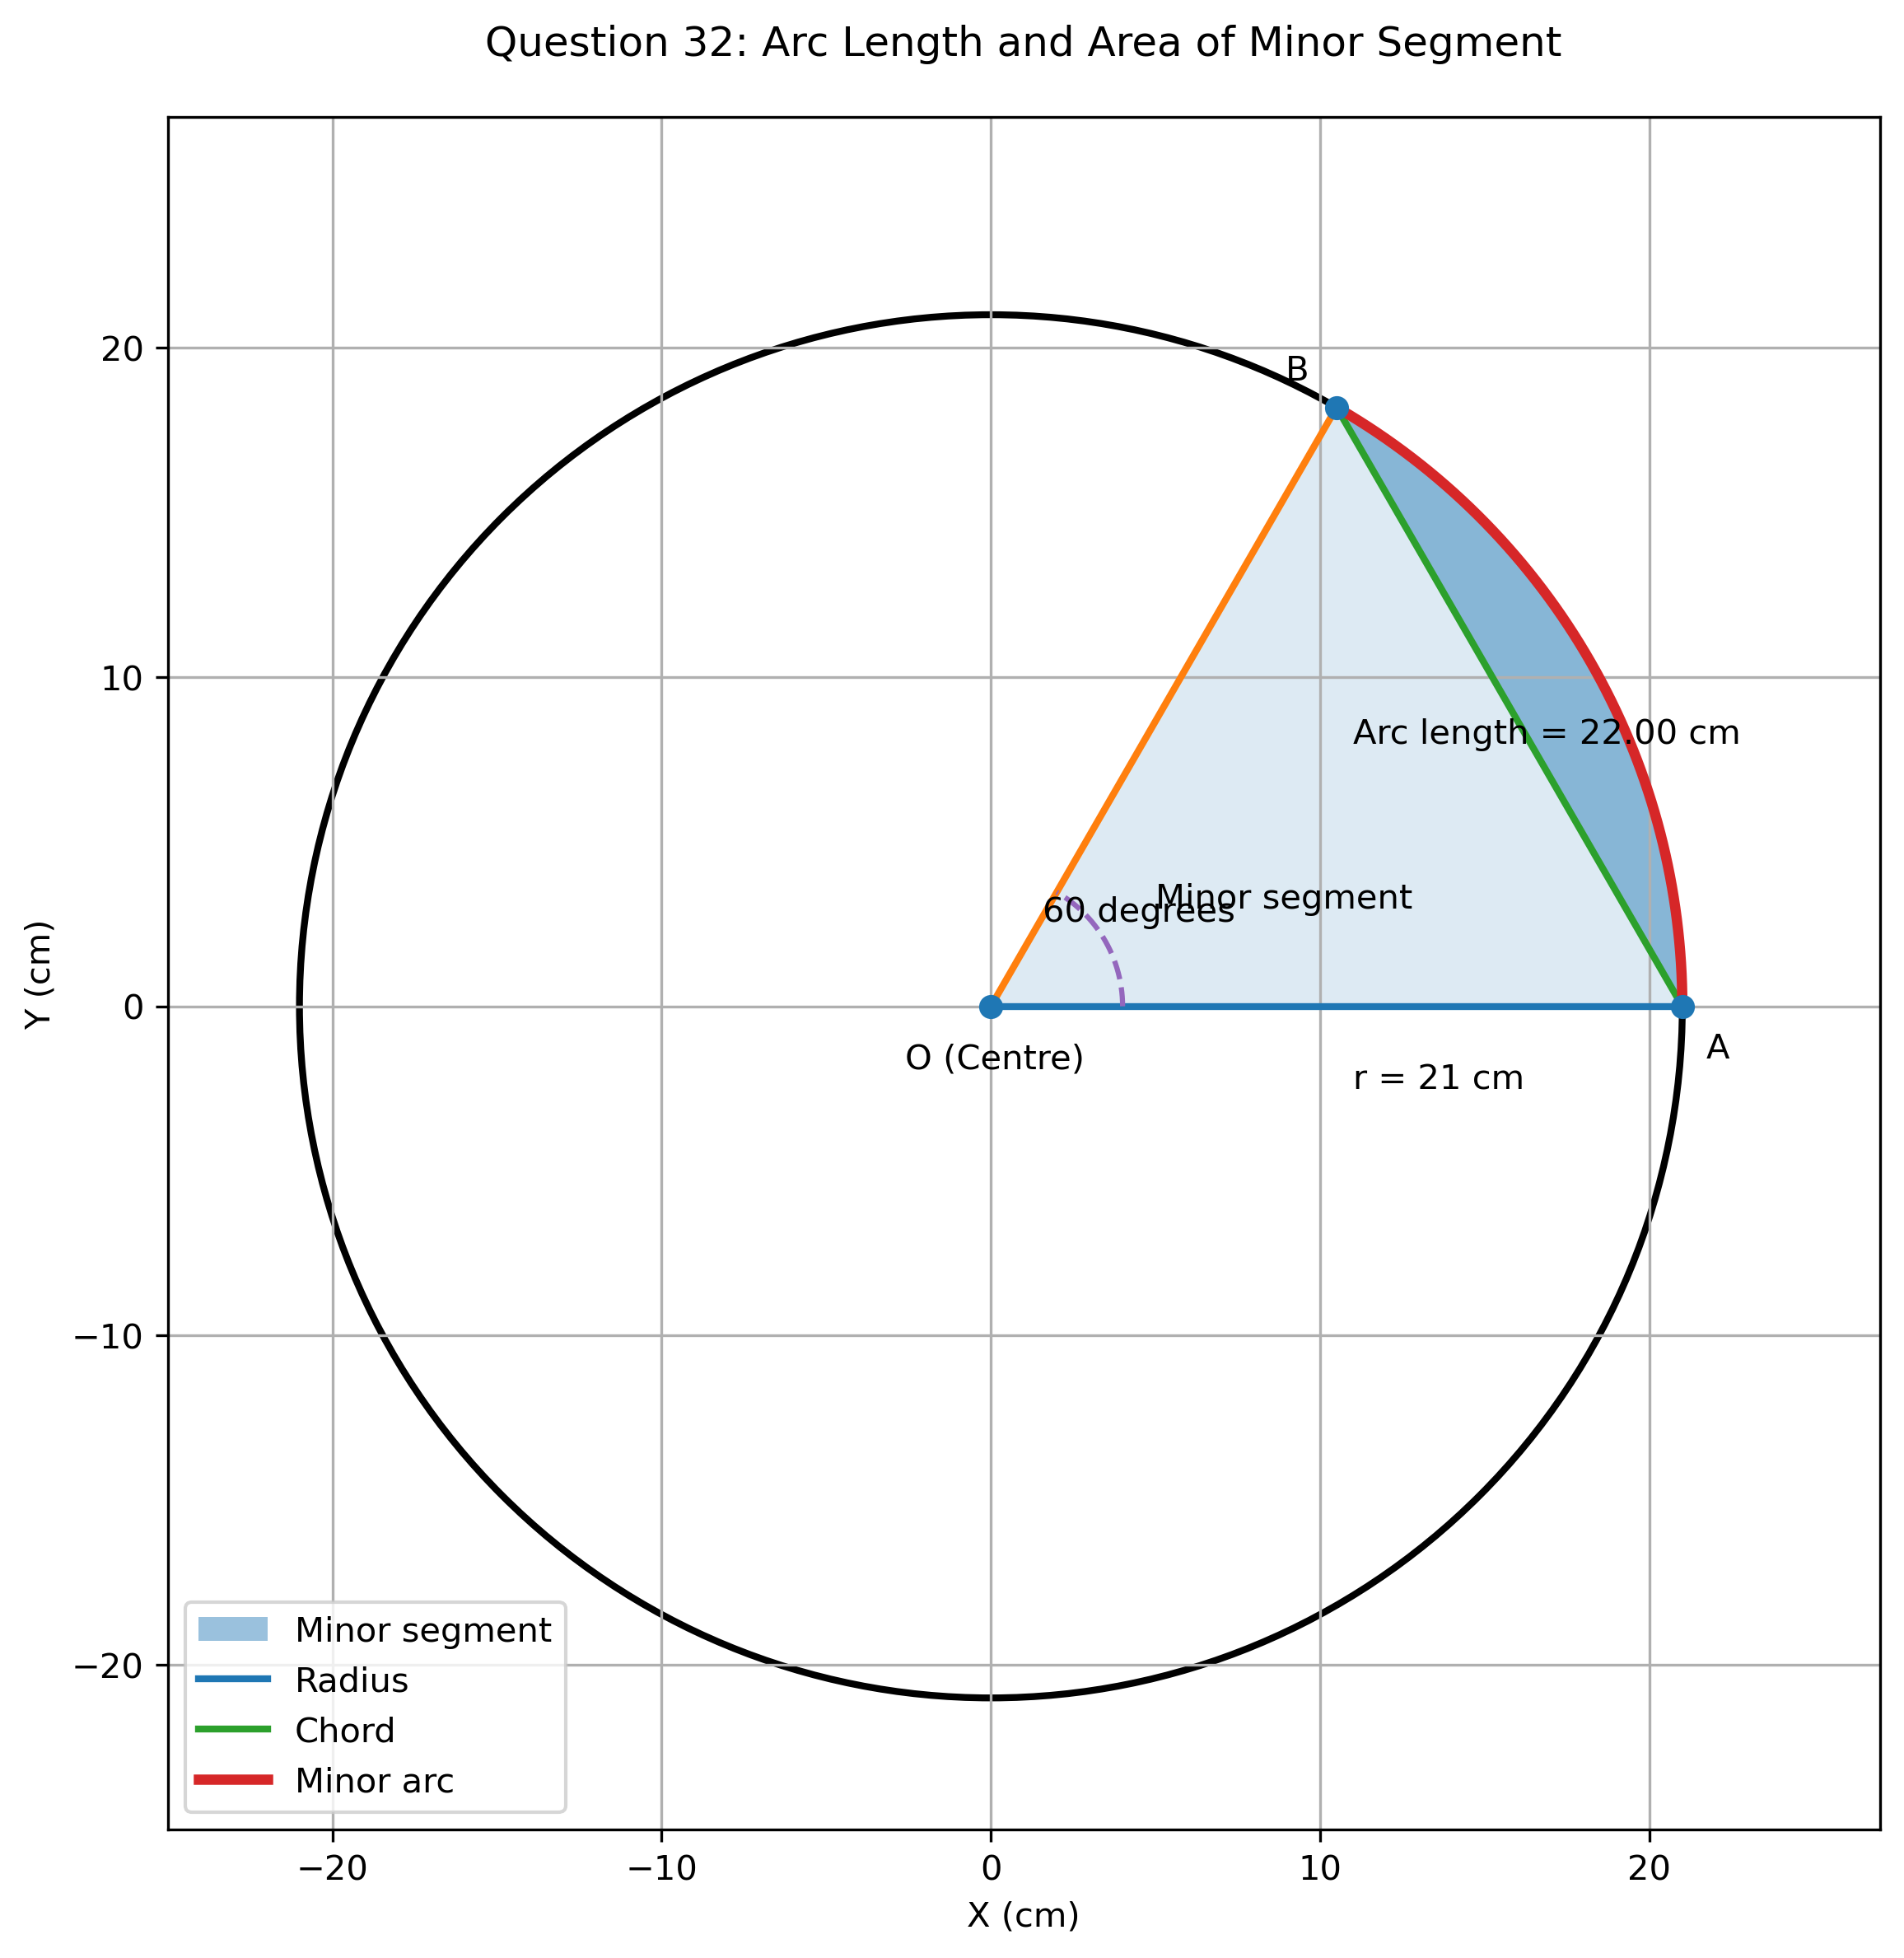
\includegraphics[
                width=0.5\textwidth,
                keepaspectratio
            ]{figs/s32.png}
        };
    \end{tikzpicture}
\end{figure}

\newpage
\item
The sum of the first and eighth terms of an A.P. is \(32\) and their product is \(60\). Find the first term and common difference of the A.P. Hence, also find the sum of its first \(20\) terms.

\solution

Let the first term be \(a\) and the common difference be \(d\).

The first term is \(a\), and the eighth term is \(a+7d\).

Given,
\begin{align}
a+\brak{a+7d}=32
\end{align}
\begin{align}
2a+7d=32 
\end{align}
Also, their product is \(60\).
\begin{align}
a\brak{a+7d}=60 
\end{align}
Let the first and eighth terms be \(x\) and \(y\), respectively.

Then,
\begin{align}
x+y=32,\qquad xy=60
\end{align}
Therefore,
\begin{align}
x\brak{32-x}=60
\end{align}
\begin{align}
\brak{x-2}\brak{x-30}=0
\end{align}

Hence,
\begin{align}
x=2 \quad \text{or} \quad x=30
\end{align}
The corresponding pairs of first and eighth terms are \(\brak{2,30}\) or \(\brak{30,2}\).

Taking the first term as \(a=2\) and the eighth term as \(a+7d=30\),
\begin{align}
2+7d=30
\end{align}
\begin{align}
a=2,\quad d=4
\end{align}
From \eqref{eq:EE26BTECH11211_Prob_2.3.10} the sum of the first \(20\) terms is
\begin{align}
S_{20}=\frac{20}{2}\sbrak{2a+\brak{20-1}d}
\end{align}
Substituting \(a=2\) and \(d=4\),
\begin{align}
S_{20}=10\sbrak{2\brak{2}+19\brak{4}}
\end{align}
\begin{align}
S_{20}=800
\end{align}

\item
 In an A.P. of \(40\) terms, the sum of the first \(9\) terms is \(153\) and the sum of the last \(6\) terms is \(687\). Determine the first term and common difference of the A.P. Also, find the sum of all the terms of the A.P.

\solution

Let the first term be \(a\) and the common difference be \(d\).

From \eqref{eq:EE26BTECH11211_Prob_2.3.10} the sum of the first \(9\) terms is
\begin{align}
S_9=\frac{9}{2}\sbrak{2a+\brak{9-1}d}
\end{align}
Given \(S_9=153\),
\begin{align}
\frac{9}{2}\brak{2a+8d}=153
\end{align}
\begin{align}
a+4d=17 \label{eq:EE26BTECH11211_Prob_34.1.10}
\end{align}
The last \(6\) terms are the \(35^\text{th}\) to \(40^\text{th}\) terms.

The \(35^\text{th}\) term is
\begin{align}
a_{35}=a+34d
\end{align}
The sum of the last \(6\) terms is
\begin{align}
687=\frac{6}{2}\sbrak{2\brak{a+34d}+\brak{6-1}d}
\end{align}
\begin{align}
2a+73d=229 \label{eq:EE26BTECH11211_Prob_34.2.10}
\end{align}
Multiplying equation \eqref{eq:EE26BTECH11211_Prob_34.1.10} by \(2\),
\begin{align}
2a+8d=34 \label{eq:EE26BTECH11211_Prob_34.3.10}
\end{align}
Subtracting equation \eqref{eq:EE26BTECH11211_Prob_34.3.10} from equation \eqref{eq:EE26BTECH11211_Prob_34.2.10},
\begin{align}
65d=195
\end{align}
\begin{align}
d=3
\end{align}
Substituting \(d=3\) in equation \eqref{eq:EE26BTECH11211_Prob_34.1.10},
\begin{align}
a+4\brak{3}=17
\end{align}
\begin{align}
a=5
\end{align}
Now, the sum of all \(40\) terms is
\begin{align}
S_{40}=\frac{40}{2}\sbrak{2a+\brak{40-1}d}
\end{align}
\begin{align}
S_{40}=2540
\end{align}

\item
 If a line is drawn parallel to one side of a triangle to intersect the other two sides at distinct points, prove that the other two sides are divided in the same ratio.

\solution
Given: In \(\triangle ABC\), let \(D\) and \(E\) be points on \(AB\) and \(AC\), respectively, such that \(DE \parallel BC\).

To prove:
\begin{align}
\frac{AD}{DB}=\frac{AE}{EC}
\end{align}
Since \(DE\parallel BC\),
\begin{align}
\triangle ADE \sim \triangle ABC
\end{align}
Therefore,
\begin{align}
\frac{AD}{AB}=\frac{AE}{AC}
\end{align}
Since \(AB=AD+DB\) and \(AC=AE+EC\),
\begin{align}
\frac{AD}{AD+DB}=\frac{AE}{AE+EC}
\end{align}
Cross-multiplying,
\begin{align}
AD\brak{AE+EC}=AE\brak{AD+DB}
\end{align}
\begin{align}
AD\cdot AE+AD\cdot EC
=AD\cdot AE+AE\cdot DB
\end{align}
Cancelling \(AD\cdot AE\) from both sides,
\begin{align}
AD\cdot EC=AE\cdot DB
\end{align}
Hence,
\begin{align}
\frac{AD}{DB}=\frac{AE}{EC}
\end{align}
Hence proved.
\\The following code generates the figure
\begin{lstlisting}[frame=single, basicstyle=\rmfamily, escapeinside={(*@}{@*)}]
(*@\makebox[\dimexpr\linewidth-2\fboxsep-2\fboxrule\relax][c]{codes/s35.py}@*)
\end{lstlisting}
\begin{figure}[ht]
    \centering

    \begin{tikzpicture}
        \node[inner sep=0pt] at (0,0)
        {
            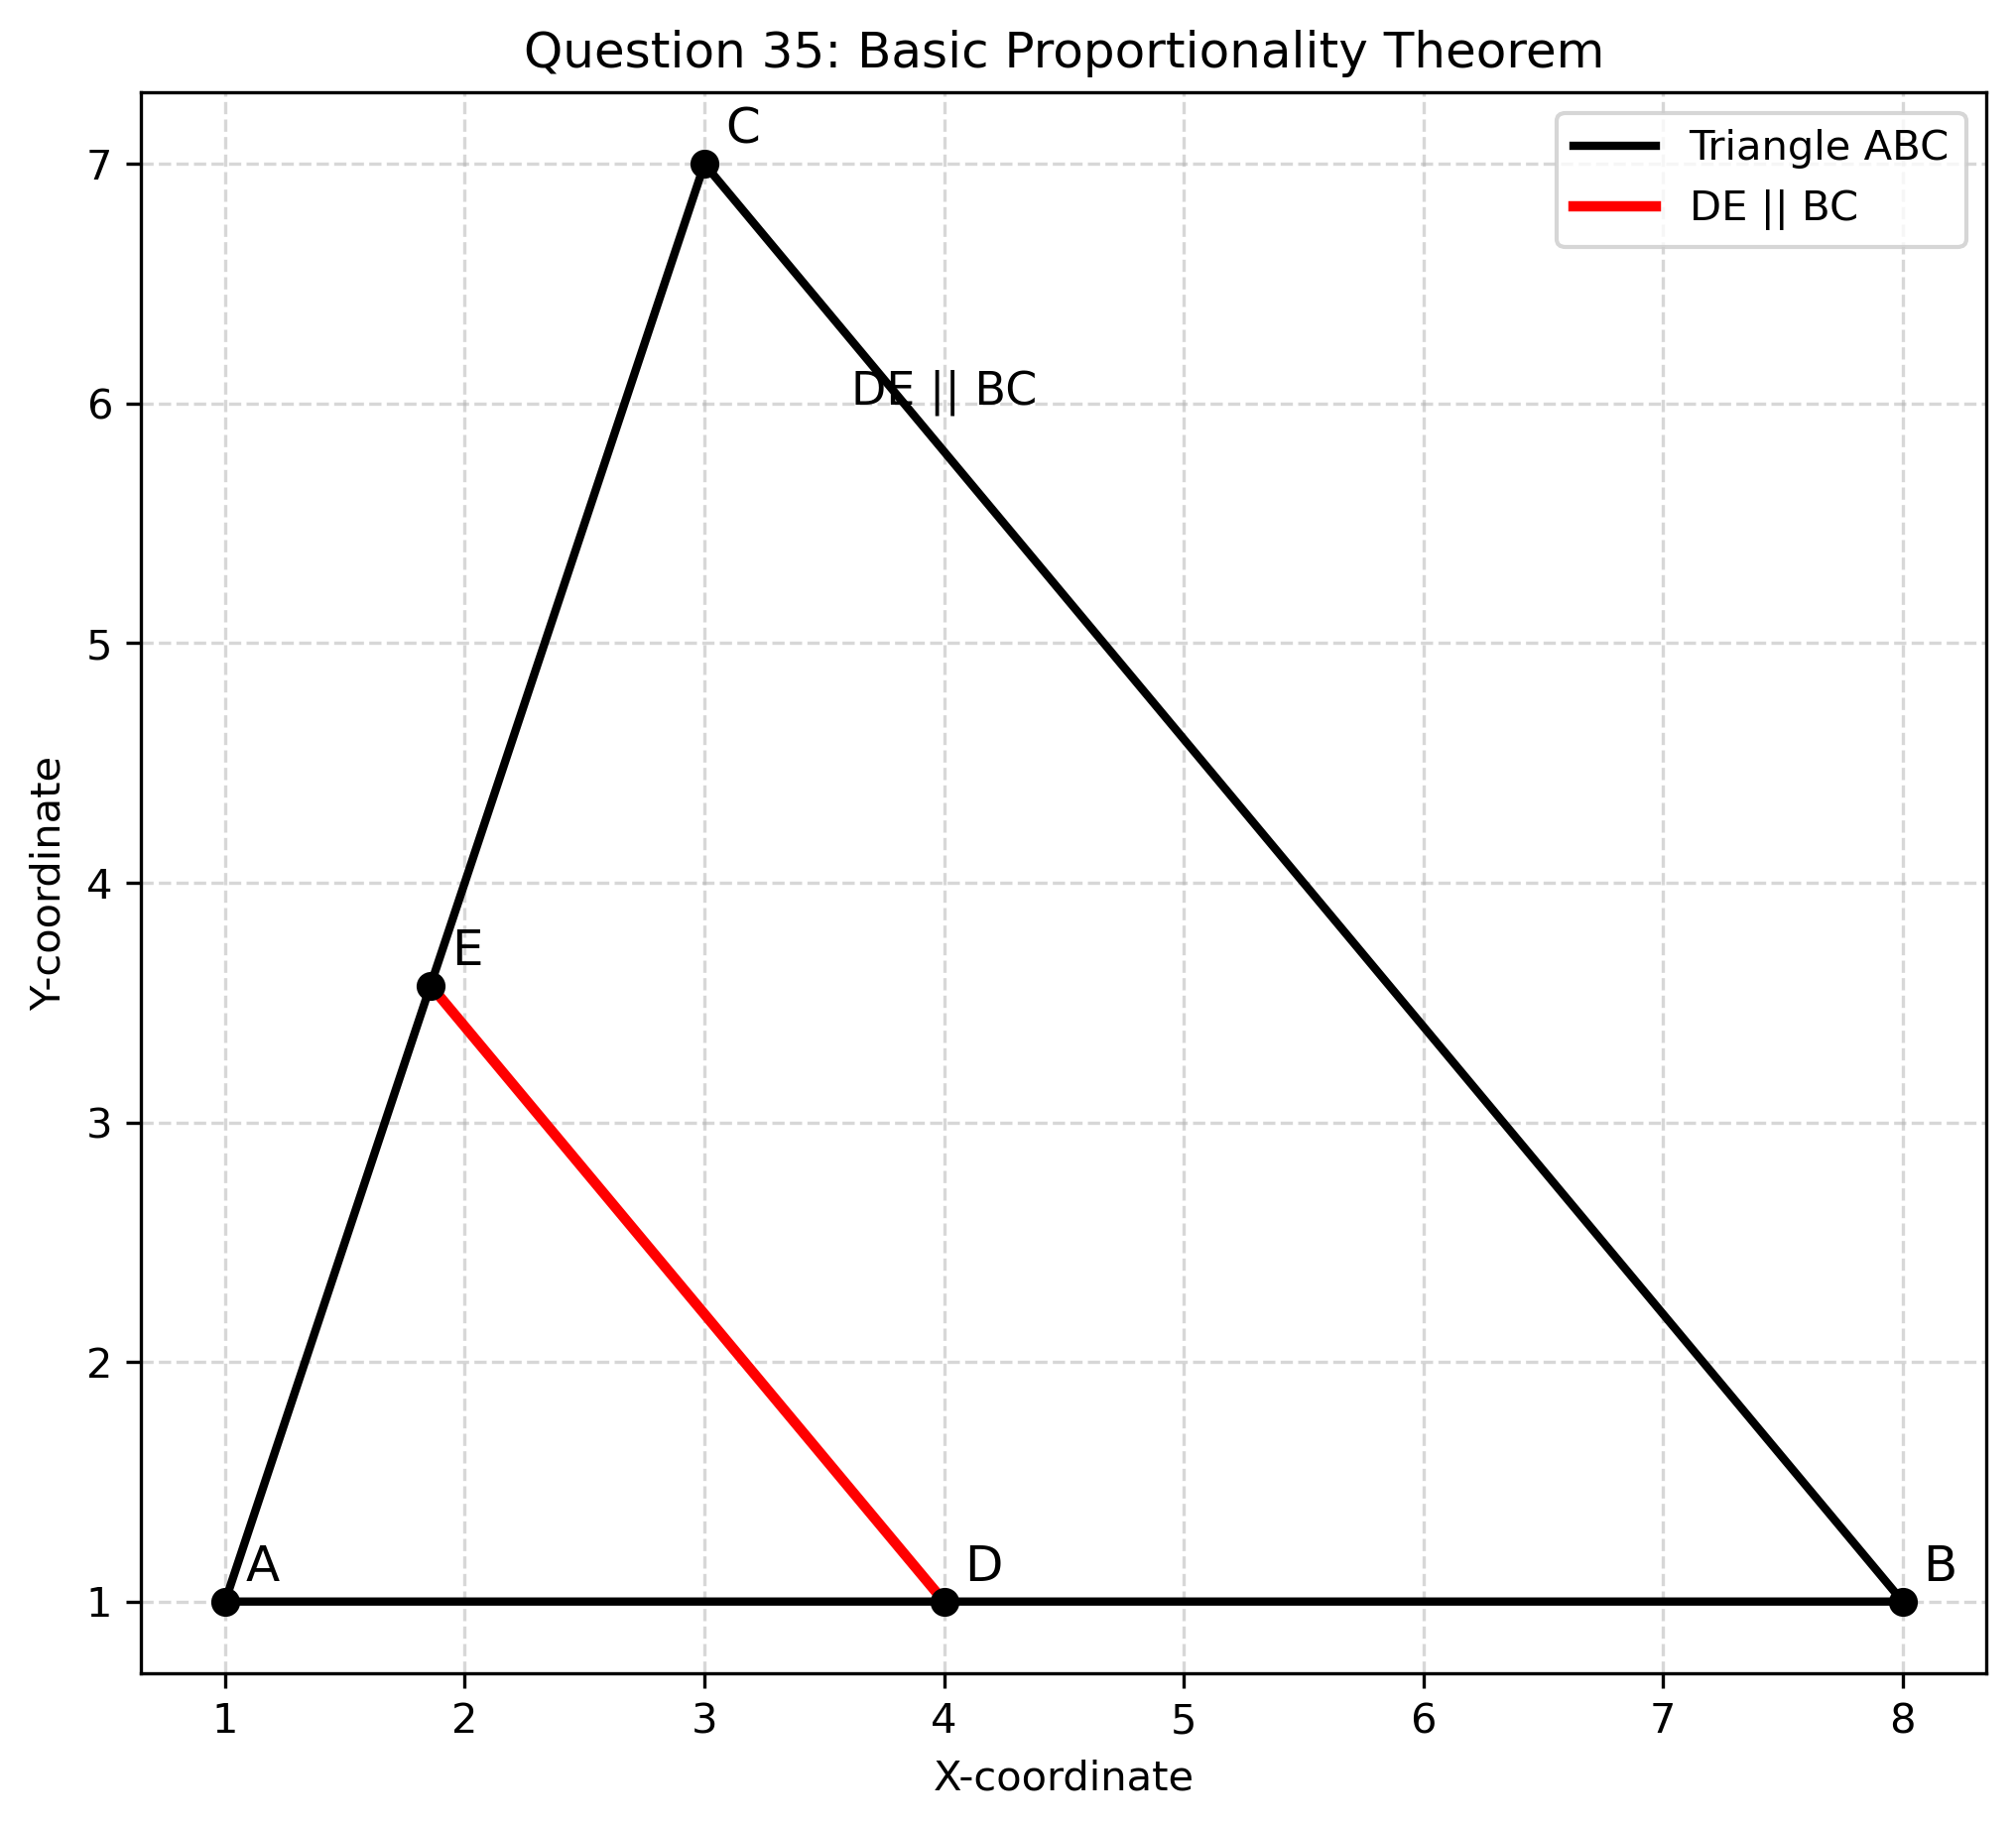
\includegraphics[
                width=0.5\textwidth,
                keepaspectratio
            ]{figs/s35.png}
        };
    \end{tikzpicture}
\end{figure}

\item
 In the given figure, \(PA\), \(QB\) and \(RC\) are perpendicular to \(AC\). If \(AP=x\), \(BQ=y\) and \(RC=z\), prove that
\begin{align}
\frac{1}{x}+\frac{1}{z}=\frac{1}{y}.
\end{align}
\begin{center}
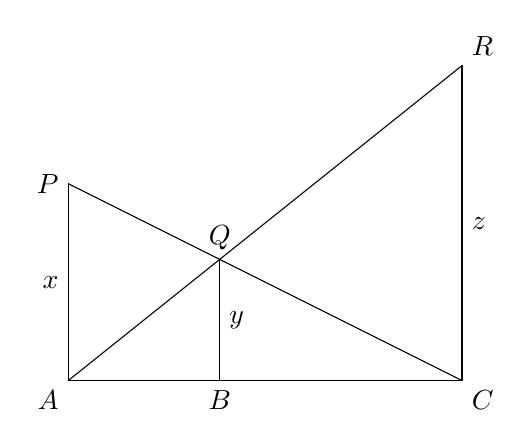
\begin{tikzpicture}[scale=1.0, line cap=round, line join=round]

    % Coordinates
    \coordinate (A) at (0,0);
    \coordinate (C) at (5,0);
    \coordinate (P) at (0,2.5);
    \coordinate (R) at (5,4);
    
    % Intersection of AR and PC
    \coordinate (Q) at (1.923,1.538);
    \coordinate (B) at (1.923,0);

    % Base AC
    \draw (A)--(C);

    % Perpendicular lines
    \draw (A)--(P);
    \draw (B)--(Q);
    \draw (C)--(R);

    % Slanting lines
    \draw (A)--(R);
    \draw (P)--(C);

    % Point labels
    \node[below left]  at (A) {$A$};
    \node[below]       at (B) {$B$};
    \node[below right] at (C) {$C$};
    \node[left]        at (P) {$P$};
    \node[above]       at (Q) {$Q$};
    \node[above right] at (R) {$R$};

    % Length labels
    \node[left] at (0,1.25) {$x$};
    \node[right] at (1.923,0.77) {$y$};
    \node[right] at (5,2) {$z$};

\end{tikzpicture}
\end{center}
\solution
From the figure, \(A,B,C\) lie on the same straight line, and \(P,Q,R\) lie as shown.
\\Since \(PA\perp AC\), \(QB\perp AC\), and \(RC\perp AC\),
\begin{align}
\angle PAQ=\angle CBQ=90^\circ
\end{align}
Also, \(\angle PQA=\angle QCB\).

Therefore,
\begin{align}
\triangle PAQ\sim\triangle CBQ
\end{align}
Hence,
\begin{align}
\frac{PA}{BC}=\frac{AQ}{CQ}
\end{align}
Similarly, using the similar triangles formed by the intersecting lines,
\begin{align}
\frac{BQ}{AP}=\frac{CQ}{AR}
\end{align}
Substituting \(AP=x\), \(BQ=y\), and \(RC=z\), we obtain
\begin{align}
\frac{1}{x}+\frac{1}{z}=\frac{1}{y}
\end{align}
Hence proved.

\item
 A tower is \(6\) m high. A point \(P\) on the ground is at a distance of \(4\) m from the foot of the tower. The angle of elevation of the top of the tower from \(P\) is \(60^\circ\). Find the height of the tower and the distance of point \(P\) from the foot of the tower. Take \(\sqrt{3}=1.73\).

\solution
Let \(AB\) be the tower and \(P\) be the point on the ground.

Given,
\begin{align}
AB=6\text{ m}, \qquad \angle APB=60^\circ
\end{align}
Using the tangent ratio,
\begin{align}
\tan 60^\circ=\frac{AB}{BP}
\end{align}
\begin{align}
BP=2\sqrt{3}
\end{align}
Using \(\sqrt{3}=1.73\),
\begin{align}
BP=3.46\text{ m}
\end{align}
The following code generates the figure
\begin{lstlisting}[frame=single, basicstyle=\rmfamily, escapeinside={(*@}{@*)}]
(*@\makebox[\dimexpr\linewidth-2\fboxsep-2\fboxrule\relax][c]{codes/s37.py}@*)
\end{lstlisting}
\begin{figure}[ht]
    \centering

    \begin{tikzpicture}
        \node[inner sep=0pt] at (0,0)
        {
            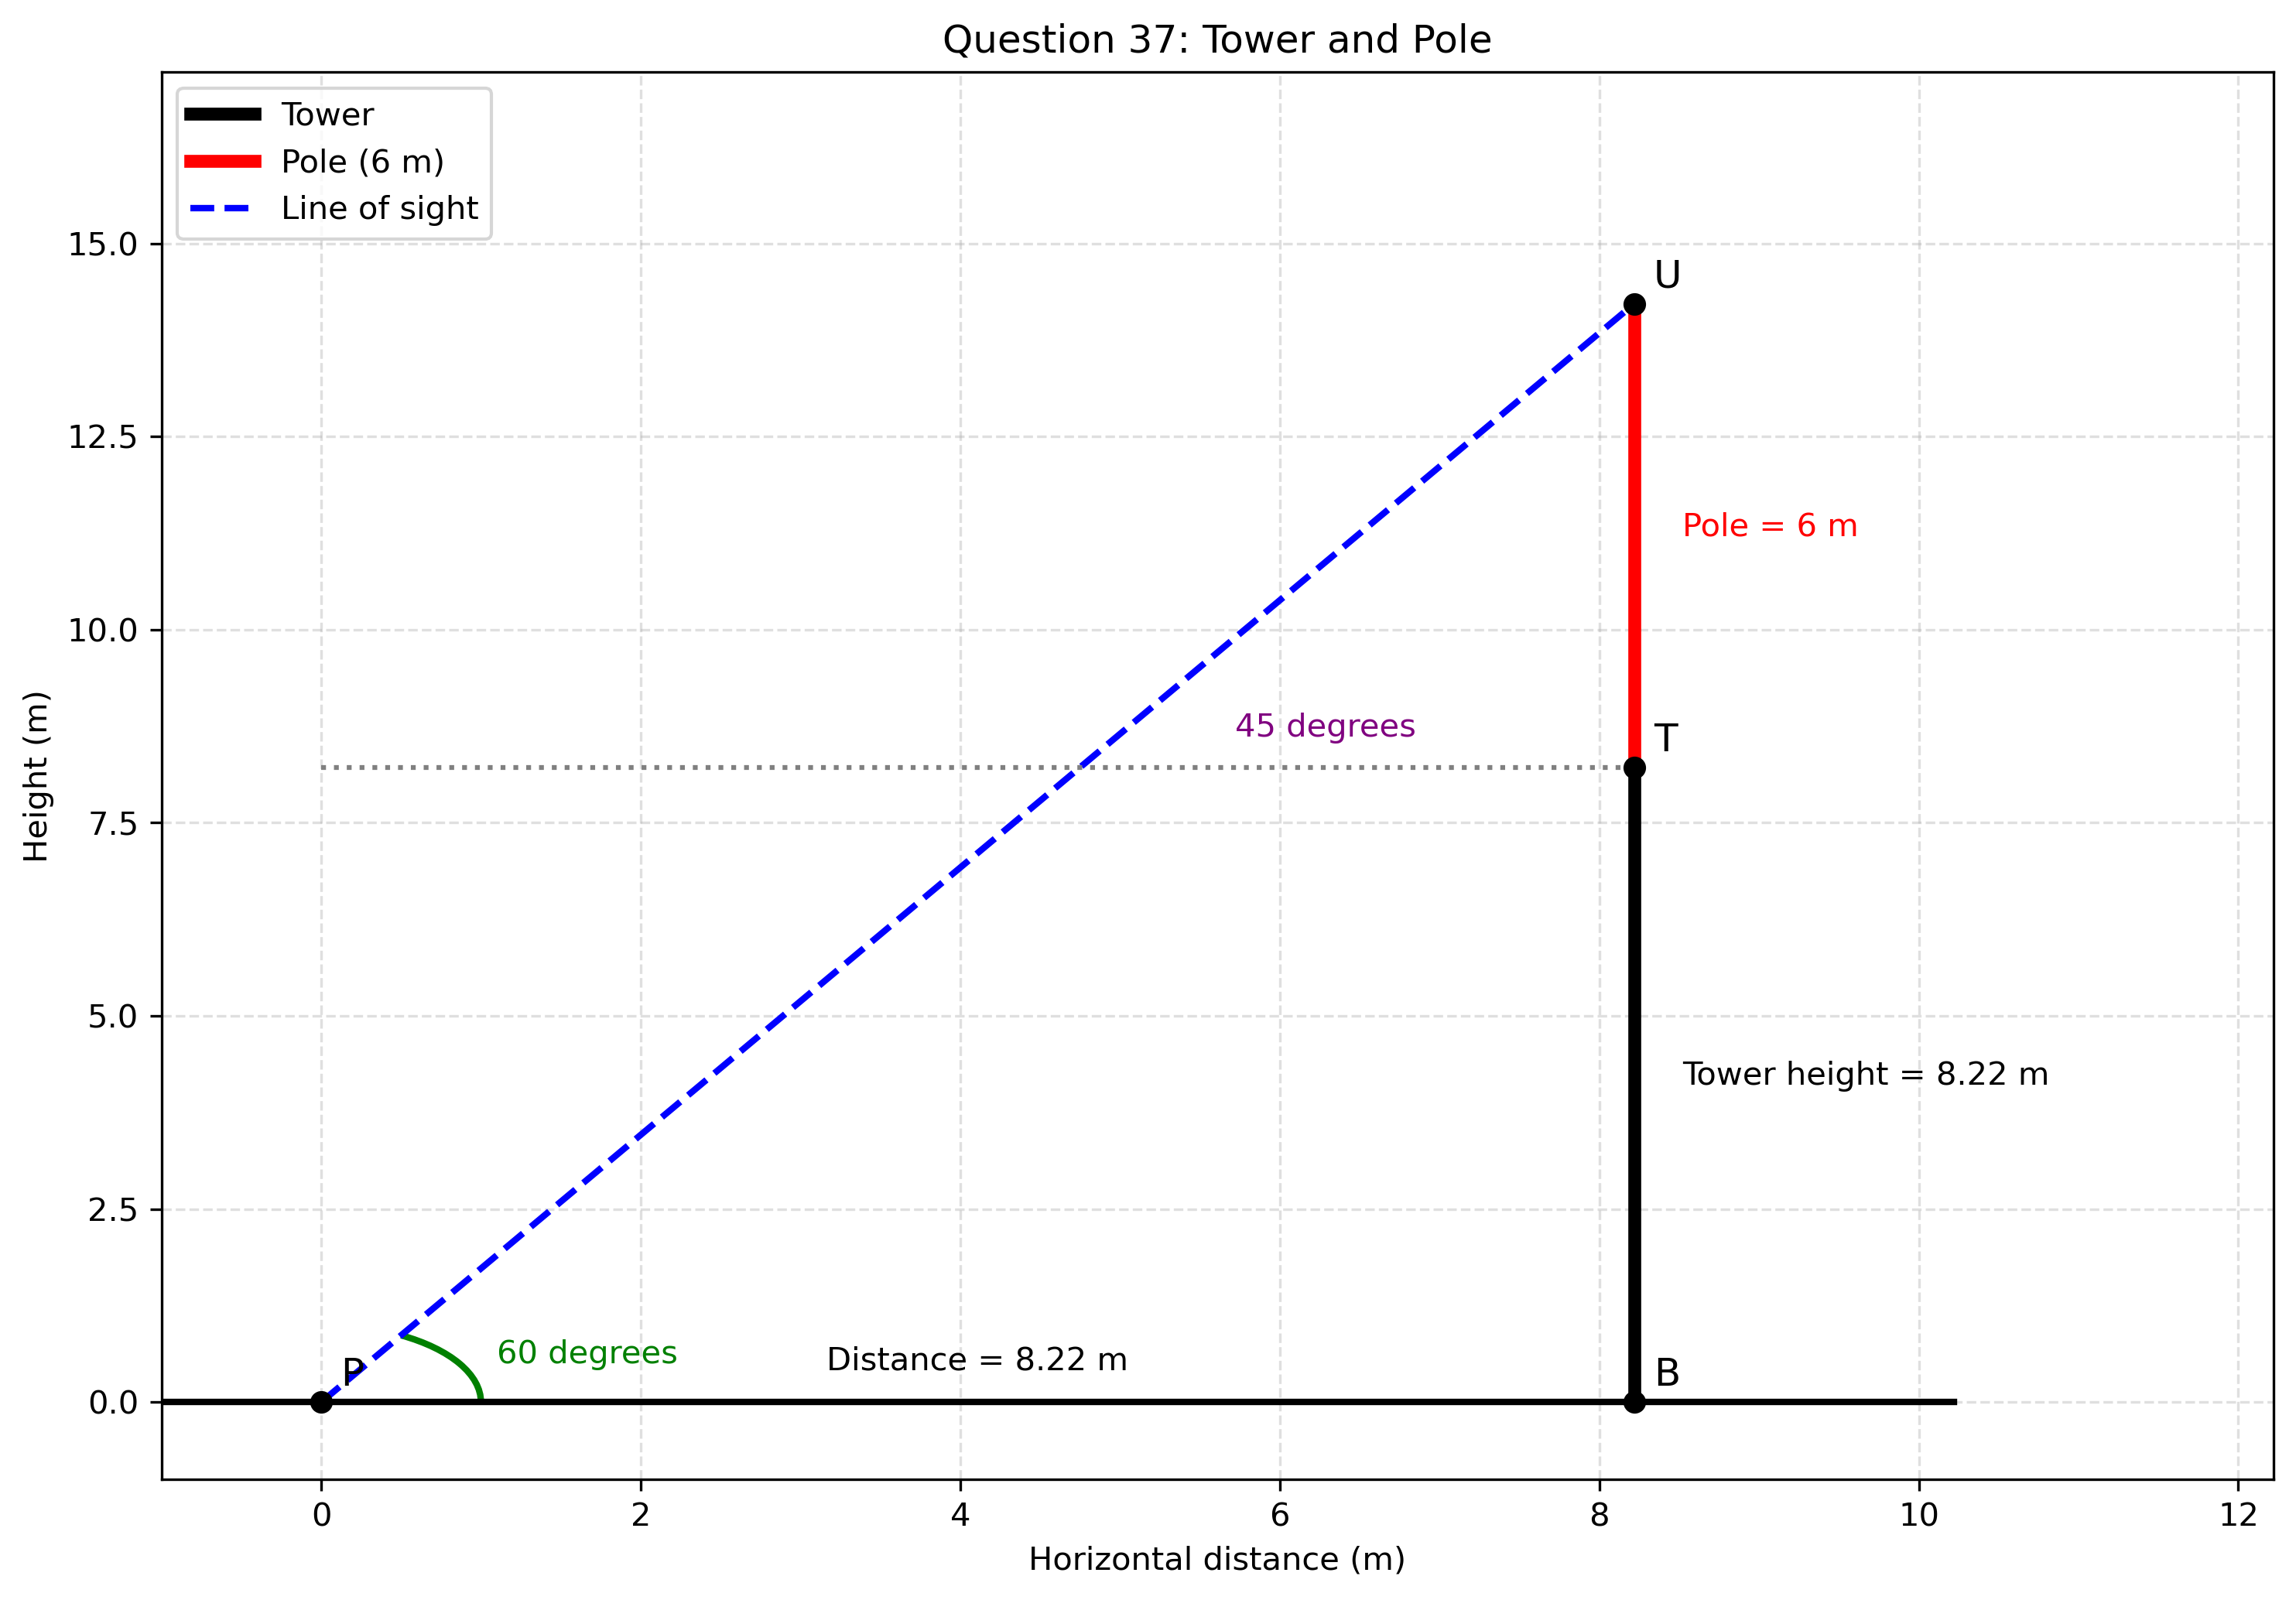
\includegraphics[
                width=0.5\textwidth,
                keepaspectratio
            ]{figs/s37.png}
        };
    \end{tikzpicture}
\end{figure}

\item
A rectangular floor area can be completely tiled with \(200\) square tiles. If the side length of each tile is increased by \(1\) unit, it would take only \(128\) tiles to cover the floor.

\begin{enumerate}
    \item[\brak{i}] Assuming the original length of each side of a tile to be \(x\) units, make a quadratic equation from the above information.
    \item[\brak{ii}] Write the corresponding quadratic equation in standard form.
    \item[\brak{iii}] \brak{a} Find the value of \(x\), the length of the side of a tile, by factorisation.
    
    OR
    
    \brak{b} Solve the quadratic equation for \(x\), using the quadratic formula.
\end{enumerate}

\begin{figure}[ht]
    \centering
    \begin{tikzpicture}
        \node[inner sep=0pt] at (0,0)
        {
            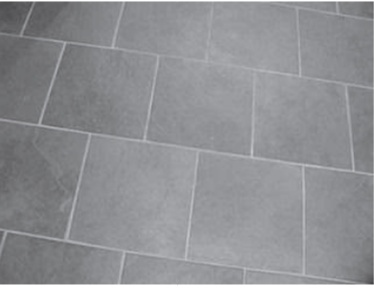
\includegraphics[
                width=0.5\textwidth,
                keepaspectratio
            ]{figs/q38.png}
        };
    \end{tikzpicture}
\end{figure}
\solution

\brak{i} Forming the quadratic equation

Let the original side length of each square tile be \(x\) units.

Area of one original tile:$x^2$

Total floor area:$200x^2$

The increased side length of each tile is \(\brak{x+1}\) units.

Area of one increased tile:

\begin{align}
\brak{x+1}^2
\end{align}

Since \(128\) increased tiles cover the same floor,

Therefore, the required quadratic equation is
\begin{align}
200x^2=128\brak{x+1}^2
\end{align}

\brak{ii} Standard form of the quadratic equation

Expanding,
\begin{align}
200x^2=128\brak{x^2+2x+1}
\end{align}
\begin{align}
72x^2-256x-128=0
\end{align}
Dividing by \(8\),
\begin{align}
9x^2-32x-16=0
\end{align}

\brak{iii} \brak{a} Solving by factorisation

The quadratic equation is
\begin{align}
9x^2-32x-16=0
\end{align}
\begin{align}
\brak{9x+4}\brak{x-4}=0
\end{align}
Therefore,
\begin{align}
9x+4=0 \quad \text{or} \quad x-4=0
\end{align}
\begin{align}
x=-\frac{4}{9} \quad \text{or} \quad x=4
\end{align}
Since the side length cannot be negative,
\begin{align}
x=4\text{ units}
\end{align}

OR

\brak{iii} \brak{b} Solving using the quadratic formula

The quadratic equation is
\begin{align}
9x^2-32x-16=0
\end{align}
Comparing with \(ax^2+bx+c=0\),
\begin{align}
a=9,\qquad b=-32,\qquad c=-16
\end{align}
Using the quadratic formula,
\begin{align}
x=\frac{-b\pm\sqrt{b^2-4ac}}{2a}
\end{align}
Substituting the values,
\begin{align}
x=\frac{32\pm\sqrt{\brak{-32}^2-4\brak{9}\brak{-16}}}{18}
\end{align}
\begin{align}
x=\frac{32\pm40}{18}
\\x= 4,-\frac{4}{9}
\end{align}
Rejecting the negative value,
\begin{align}
x=4\text{ units}
\end{align}

\item
 BINGO is a game of chance. The host has \(75\) balls numbered \(1\) through \(75\). Each player has a BINGO card with some numbers written on it. The participant cancels the number on the card when a number written on the ball selected at random is called out. Whoever cancels all the numbers on their card first says BINGO and wins the game.
 \begin{figure}[ht]
    \centering
    \begin{tikzpicture}
        \node[inner sep=0pt] at (0,0)
        {
            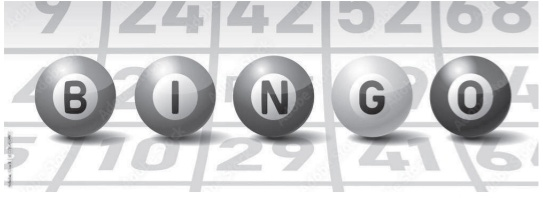
\includegraphics[
                width=\textwidth,
                keepaspectratio
            ]{figs/q39.png}
        };
    \end{tikzpicture}
\end{figure}
The following frequency distribution shows the numbers called out before a player says BINGO:

\begin{center}
\begin{tabular}{|c|c|}
\hline
Number on the ball & Frequency \\
\hline
\(0-15\) & \(8\) \\
\hline
\(15-30\) & \(9\) \\
\hline
\(30-45\) & \(10\) \\
\hline
\(45-60\) & \(12\) \\
\hline
\(60-75\) & \(9\) \\
\hline
\end{tabular}
\end{center}

Answer the following questions based on the above information:

\begin{enumerate}
    \item[\brak{i}] Write the median class.
    \item[\brak{ii}] What is the probability of calling an even number when the first ball is drawn?
    \item[\brak{iii}] \brak{a} Find the median of the given data.
    
    OR
    
    \brak{b} Find the mode of the given data.
\end{enumerate}

\solution

\brak{i} Median class

The frequencies are

\begin{align}
8,\ 9,\ 10,\ 12,\ 9
\end{align}
The cumulative frequency table is:

\begin{center}
\begin{tabular}{|c|c|c|}
\hline
Class interval & Frequency & Cumulative frequency \\
\hline
\(0-15\) & \(8\) & \(8\) \\
\hline
\(15-30\) & \(9\) & \(17\) \\
\hline
\(30-45\) & \(10\) & \(27\) \\
\hline
\(45-60\) & \(12\) & \(39\) \\
\hline
\(60-75\) & \(9\) & \(48\) \\
\hline
\end{tabular}
\end{center}

Total frequency:
\begin{align}
N=48
\end{align}
\begin{align}
\frac{N}{2}=\frac{48}{2}=24
\end{align}
The cumulative frequency immediately greater than \(24\) is \(27\), corresponding to the class \(30-45\).

Therefore,
\begin{align}
\text{Median class}=30-45
\end{align}

\brak{ii} Probability of calling an even number

There are \(75\) balls numbered from \(1\) to \(75\).

The number of even numbers is \(37\).

Therefore,
\begin{align}
P\brak{\text{even number}}
=\frac{\text{Number of even numbers}}{\text{Total number of balls}}
\end{align}
\begin{align}
P\brak{\text{even number}}=\frac{37}{75}
\end{align}
\brak{iii} \brak{a} Median of the given data

From \eqref{eq:EE26BTECH11211_Prob_3.16.10} the formula for the median of grouped data is
\begin{align}
\text{Median}=l+\brak{\frac{\frac{N}{2}-cf}{f}}h
\end{align}
Here,
\begin{align}
l=30,\quad N=48,\quad cf=17,\quad f=10,\quad h=15
\end{align}
Substituting these values,
\begin{align}
\text{Median}
=30+\brak{\frac{24-17}{10}}15
\end{align}
\begin{align}
\text{Median}=40.5
\end{align}
OR

\brak{iii} \brak{b} Mode of the given data

The modal class is the class with the highest frequency.

The highest frequency is \(12\), so the modal class is \(45-60\).

From \eqref{eq:EE26BTECH11211_Prob_3.17.10} the formula for the mode of grouped data is
\begin{align}
\text{Mode}
=l+\brak{\frac{f_1-f_0}{2f_1-f_0-f_2}}h
\end{align}
Here,
\begin{align}
l=45,\quad f_1=12,\quad f_0=10,\quad f_2=9,\quad h=15
\end{align}
Substituting the values,
\begin{align}
\text{Mode}
=45+\brak{\frac{12-10}{2\brak{12}-10-9}}15
\end{align}
\begin{align}
\text{Mode}=51
\end{align}

\item
A backyard is in the shape of a triangle \(ABC\) with a right angle at \(B\). \(AB=7\text{ m}\) and \(BC=15\text{ m}\). A circular pit was dug inside it such that it touches the walls \(AC\), \(BC\), and \(AB\) at \(P\), \(Q\), and \(R\), respectively, such that \(AP=x\text{ m}\).
\begin{figure}[ht]
    \centering
    \begin{tikzpicture}
        \node[inner sep=0pt] at (0,0)
        {
            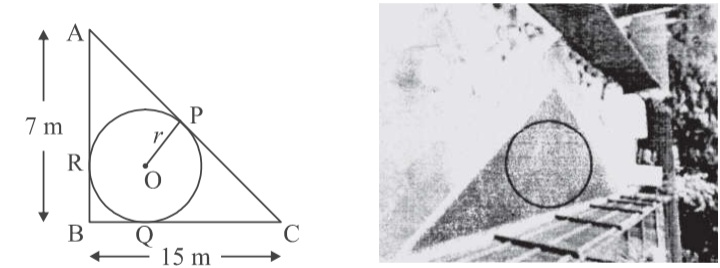
\includegraphics[
                width=\textwidth,
                keepaspectratio
            ]{figs/q40.png}
        };
    \end{tikzpicture}
\end{figure}
Based on the above information, answer the following questions:

\begin{enumerate}
    \item[\brak{i}] Find the length of \(AR\) in terms of \(x\).
    \item[\brak{ii}] Write the type of quadrilateral \(BQOR\).
    \item[\brak{iii}] \brak{a} Find the length \(PC\) in terms of \(x\) and hence find the value of \(x\).

    OR

    \brak{b} Find \(x\) and hence find the radius \(r\) of the circle.
\end{enumerate}

\solution

\brak{i} Find the length of \(AR\) in terms of \(x\)

Tangents drawn from an external point to a circle are equal.

From point \(A\),
\begin{align}
AP=AR
\end{align}
Given \(AP=x\text{ m}\),
\begin{align}
AR=x\text{ m} \label{eq:EE26BTECH11211_Prob_40.1.10}
\end{align}
\brak{ii} Write the type of quadrilateral \(BQOR\)

Since the radius is perpendicular to the tangent at the point of contact,
\begin{align}
\angle BQO=90^\circ
\end{align}
\begin{align}
\angle BRO=90^\circ
\end{align}

Also, \(BQ=BR\) because tangents drawn from \(B\) are equal, and \(OQ=OR\) because both are radii.

Therefore, \(BQOR\) is a square.

\brak{iii} \brak{a} Find \(PC\) in terms of \(x\) and hence find \(x\)

Tangents drawn from point \(C\) are equal.

Therefore,
\begin{align}
CP=CQ
\end{align}
From \eqref{eq:EE26BTECH11211_Prob_40.1.10},
\begin{align}
AB=AR+RB
\end{align}
\begin{align}
RB=7-x
\end{align}
Since tangents drawn from \(B\) are equal,
\begin{align}
BQ=BR=7-x  \label{eq:EE26BTECH11211_Prob_40.2.10}
\end{align}
Now,
\begin{align}
BC=BQ+QC
\end{align}
\begin{align}
QC=8+x
\end{align}
Since \(CP=CQ\),
\begin{align}
PC=x+8\text{ m}
\end{align}
Using the Pythagorean theorem in right-angled triangle \(ABC\),
\begin{align}
AC^2=AB^2+BC^2
\end{align}
\begin{align}
AC=\sqrt{274}\text{ m}
\end{align}
Also,
\begin{align}
AC=AP+PC
\end{align}
\begin{align}
x=\frac{\sqrt{274}-8}{2}\text{ m}
\end{align}

OR

\brak{iii} \brak{b} Find \(x\) and hence find the radius \(r\) of the circle

From the above result,
\begin{align}
x=\frac{\sqrt{274}-8}{2}\text{ m}
\end{align}
Since \(OQ\) is the radius and \(BQOR\) is a square,
\begin{align}
r=BQ
\end{align}
From \eqref{eq:EE26BTECH11211_Prob_40.2.10},
$BQ=7-x$

Therefore,
\begin{align}
r=7-\frac{\sqrt{274}-8}{2}
\end{align}
\begin{align}
r=\frac{22-\sqrt{274}}{2}\text{ m}
\end{align}

\end{enumerate}